% A LaTeX (non-official) template for ISAE projects reports
% Copyright (C) 2014 Damien Roque
% Version: 0.2
% Author: Damien Roque <damien.roque_AT_isae.fr>

% Template adapted for English reports by:
% Johannes Wasmer (JW)

\documentclass[a4paper,12pt, openany]{book} %openany: chapters start on any
                                %page, not just odd pages (which creates blank pages)
\usepackage[utf8]{inputenc}
\usepackage[T1]{fontenc}


%%%%%%%%%%%%%%%%%%%%%%%%%%%%%%%%%%%%% 
%%%%%%%%%% TEMPLATE CONFIG %%%%%%%%%%
%%%%%%%%%%%%%%%%%%%%%%%%%%%%%%%%%%%%% 

\renewcommand{\familydefault}{\sfdefault} % use sans serif font for whole document

% \usepackage[frenchb]{babel} % If you write in French
\usepackage[english]{babel} % If you write in English


\usepackage[                    % adapted template: use biber
backend=biber,                  % instead of biblatex
style=alphabetic,
citestyle=authoryear
]{biblatex}
\addbibresource{references.bib} %Imports bibliography file

\usepackage{a4wide}
\usepackage{graphicx}
\graphicspath{{./fig/}{./img/}}
\usepackage{subfig}
\usepackage{tikz}
\usetikzlibrary{shapes,arrows}
\usepackage{pgfplots}
\pgfplotsset{compat=newest}
\pgfplotsset{plot coordinates/math parser=false}
\newlength\figureheight
\newlength\figurewidth
\pgfkeys{/pgf/number format/.cd,
  set decimal separator={,\!},
  1000 sep={\,},
}
\usepackage{ifthen}
\usepackage{ifpdf}
\ifpdf
\usepackage[pdftex]{hyperref}
\else
\usepackage{hyperref}
\fi
\usepackage{color}
\hypersetup{%
  colorlinks=true,
  linkcolor=black,
  citecolor=black,
  urlcolor=black}

\renewcommand{\baselinestretch}{1.05}
\usepackage{fancyhdr}
\pagestyle{fancy}
\fancyfoot{}
\fancyhead[LE,RO]{\bfseries\thepage}
\fancyhead[RE]{\bfseries\nouppercase{\leftmark}}
\fancyhead[LO]{\bfseries\nouppercase{\rightmark}}
\setlength{\headheight}{15pt}

\let\headruleORIG\headrule
\renewcommand{\headrule}{\color{black} \headruleORIG}
\renewcommand{\headrulewidth}{1.0pt}
\usepackage{colortbl}
\arrayrulecolor{black}

\fancypagestyle{plain}{
  \fancyhead{}
  \fancyfoot[C]{\thepage}
  \renewcommand{\headrulewidth}{0pt}
}

\makeatletter
\def\@textbottom{\vskip \z@ \@plus 1pt}
\let\@texttop\relax
\makeatother

\makeatletter
\def\cleardoublepage{\clearpage\if@twoside \ifodd\c@page\else%
  \hbox{}%
  \thispagestyle{empty}%
  \newpage%
  \if@twocolumn\hbox{}\newpage\fi\fi\fi}
\makeatother

\usepackage{amsthm}
\usepackage{amssymb,amsmath,bbm}
\usepackage{array}
\usepackage{bm}
\usepackage{multirow}
\usepackage[footnote]{acronym}


%%%%%%%%%%%%%%%%%%%%%%%%%%%%%%%%%%%%%
%%%%%%%%%% CONFIG JOHANNES %%%%%%%%%%
%%%%%%%%%%%%%%%%%%%%%%%%%%%%%%%%%%%%%

\usepackage{fontawesome}
\usepackage{dashrule}
\usepackage{hyperref}
\hypersetup{
  colorlinks,
  linkcolor={red!50!black},
  citecolor={blue!50!black},
  urlcolor={blue!80!black}
}



%%% Local Variables:
%%% mode: latex
%%% TeX-master: "../report"
%%% End:



\newcommand*{\SET}[1]  {\ensuremath{\mathbf{#1}}}
\newcommand*{\VEC}[1]  {\ensuremath{\boldsymbol{#1}}}
\newcommand*{\FAM}[1]  {\ensuremath{\boldsymbol{#1}}}
\newcommand*{\MAT}[1]  {\ensuremath{\boldsymbol{#1}}}
\newcommand*{\OP}[1]  {\ensuremath{\mathrm{#1}}}
\newcommand*{\NORM}[1]  {\ensuremath{\left\|#1\right\|}}
\newcommand*{\DPR}[2]  {\ensuremath{\left \langle #1,#2 \right \rangle}}
\newcommand*{\calbf}[1]  {\ensuremath{\boldsymbol{\mathcal{#1}}}}
\newcommand*{\shift}[1]  {\ensuremath{\boldsymbol{#1}}}

\newcommand{\eqdef}{\stackrel{\mathrm{def}}{=}}
\newcommand{\argmax}{\operatornamewithlimits{argmax}}
\newcommand{\argmin}{\operatornamewithlimits{argmin}}
\newcommand{\ud}{\, \mathrm{d}}
\newcommand{\vect}{\text{Vect}}
\newcommand{\sinc}{\ensuremath{\mathrm{sinc}}}
\newcommand{\esp}{\ensuremath{\mathbb{E}}}
\newcommand{\hilbert}{\ensuremath{\mathcal{H}}}
\newcommand{\fourier}{\ensuremath{\mathcal{F}}}
\newcommand{\sgn}{\text{sgn}}
\newcommand{\intTT}{\int_{-T}^{T}}
\newcommand{\intT}{\int_{-\frac{T}{2}}^{\frac{T}{2}}}
\newcommand{\intinf}{\int_{-\infty}^{+\infty}}
\newcommand{\Sh}{\ensuremath{\boldsymbol{S}}}
\newcommand{\C}{\SET{C}}
\newcommand{\R}{\SET{R}}
\newcommand{\Z}{\SET{Z}}
\newcommand{\N}{\SET{N}}
\newcommand{\K}{\SET{K}}
\newcommand{\reel}{\mathcal{R}}
\newcommand{\imag}{\mathcal{I}}
\newcommand{\cmnr}{c_{m,n}^\reel}
\newcommand{\cmni}{c_{m,n}^\imag}
\newcommand{\cnr}{c_{n}^\reel}
\newcommand{\cni}{c_{n}^\imag}
\newcommand{\tproto}{g}
\newcommand{\rproto}{\check{g}}
\newcommand{\LR}{\mathcal{L}_2(\SET{R})}
\newcommand{\LZ}{\ell_2(\SET{Z})}
\newcommand{\LZI}[1]{\ell_2(\SET{#1})}
\newcommand{\LZZ}{\ell_2(\SET{Z}^2)}
\newcommand{\diag}{\operatorname{diag}}
\newcommand{\noise}{z}
\newcommand{\Noise}{Z}
\newcommand{\filtnoise}{\zeta}
\newcommand{\tp}{g}
\newcommand{\rp}{\check{g}}
\newcommand{\TP}{G}
\newcommand{\RP}{\check{G}}
\newcommand{\dmin}{d_{\mathrm{min}}}
\newcommand{\Dmin}{D_{\mathrm{min}}}
\newcommand{\Image}{\ensuremath{\text{Im}}}
\newcommand{\Span}{\ensuremath{\text{Span}}}

\newtheoremstyle{break}
{11pt}{11pt}%
{\itshape}{}%
{\bfseries}{}%
{\newline}{}%
\theoremstyle{break}

% \theoremstyle{definition}
\newtheorem{definition}{Definition}[chapter]

% \theoremstyle{definition}
\newtheorem{theorem}{Theorem}[chapter] % lemma < proposition < theorem

% \theoremstyle{remark}
\newtheorem{remark}{Remark}[chapter]

% \theoremstyle{plain}
\newtheorem{property}{Property}[chapter]
\newtheorem{example}{Example}[chapter]


%%% Local Variables:
%%% mode: latex
%%% TeX-master: "report"
%%% End:

%% This is the config for the TeXified version of the README.md that makes up
%% Chapter 4 (Manual). It is the result of the command 'pandoc -s README.md -o README.tex'.


\usepackage{fancyvrb}
\newcommand{\VerbBar}{|}
\newcommand{\VERB}{\Verb[commandchars=\\\{\}]}
\DefineVerbatimEnvironment{Highlighting}{Verbatim}{commandchars=\\\{\}}
% Add ',fontsize=\small' for more characters per line
\newenvironment{Shaded}{}{}
\newcommand{\KeywordTok}[1]{\textcolor[rgb]{0.00,0.44,0.13}{\textbf{#1}}}
\newcommand{\DataTypeTok}[1]{\textcolor[rgb]{0.56,0.13,0.00}{#1}}
\newcommand{\DecValTok}[1]{\textcolor[rgb]{0.25,0.63,0.44}{#1}}
\newcommand{\BaseNTok}[1]{\textcolor[rgb]{0.25,0.63,0.44}{#1}}
\newcommand{\FloatTok}[1]{\textcolor[rgb]{0.25,0.63,0.44}{#1}}
\newcommand{\ConstantTok}[1]{\textcolor[rgb]{0.53,0.00,0.00}{#1}}
\newcommand{\CharTok}[1]{\textcolor[rgb]{0.25,0.44,0.63}{#1}}
\newcommand{\SpecialCharTok}[1]{\textcolor[rgb]{0.25,0.44,0.63}{#1}}
\newcommand{\StringTok}[1]{\textcolor[rgb]{0.25,0.44,0.63}{#1}}
\newcommand{\VerbatimStringTok}[1]{\textcolor[rgb]{0.25,0.44,0.63}{#1}}
\newcommand{\SpecialStringTok}[1]{\textcolor[rgb]{0.73,0.40,0.53}{#1}}
\newcommand{\ImportTok}[1]{#1}
\newcommand{\CommentTok}[1]{\textcolor[rgb]{0.38,0.63,0.69}{\textit{#1}}}
\newcommand{\DocumentationTok}[1]{\textcolor[rgb]{0.73,0.13,0.13}{\textit{#1}}}
\newcommand{\AnnotationTok}[1]{\textcolor[rgb]{0.38,0.63,0.69}{\textbf{\textit{#1}}}}
\newcommand{\CommentVarTok}[1]{\textcolor[rgb]{0.38,0.63,0.69}{\textbf{\textit{#1}}}}
\newcommand{\OtherTok}[1]{\textcolor[rgb]{0.00,0.44,0.13}{#1}}
\newcommand{\FunctionTok}[1]{\textcolor[rgb]{0.02,0.16,0.49}{#1}}
\newcommand{\VariableTok}[1]{\textcolor[rgb]{0.10,0.09,0.49}{#1}}
\newcommand{\ControlFlowTok}[1]{\textcolor[rgb]{0.00,0.44,0.13}{\textbf{#1}}}
\newcommand{\OperatorTok}[1]{\textcolor[rgb]{0.40,0.40,0.40}{#1}}
\newcommand{\BuiltInTok}[1]{#1}
\newcommand{\ExtensionTok}[1]{#1}
\newcommand{\PreprocessorTok}[1]{\textcolor[rgb]{0.74,0.48,0.00}{#1}}
\newcommand{\AttributeTok}[1]{\textcolor[rgb]{0.49,0.56,0.16}{#1}}
\newcommand{\RegionMarkerTok}[1]{#1}
\newcommand{\InformationTok}[1]{\textcolor[rgb]{0.38,0.63,0.69}{\textbf{\textit{#1}}}}
\newcommand{\WarningTok}[1]{\textcolor[rgb]{0.38,0.63,0.69}{\textbf{\textit{#1}}}}
\newcommand{\AlertTok}[1]{\textcolor[rgb]{1.00,0.00,0.00}{\textbf{#1}}}
\newcommand{\ErrorTok}[1]{\textcolor[rgb]{1.00,0.00,0.00}{\textbf{#1}}}
\newcommand{\NormalTok}[1]{#1}
\usepackage{graphicx,grffile}
\makeatletter
\def\maxwidth{\ifdim\Gin@nat@width>\linewidth\linewidth\else\Gin@nat@width\fi}
\def\maxheight{\ifdim\Gin@nat@height>\textheight\textheight\else\Gin@nat@height\fi}
\makeatother
% Scale images if necessary, so that they will not overflow the page
% margins by default, and it is still possible to overwrite the defaults
% using explicit options in \includegraphics[width, height, ...]{}
\setkeys{Gin}{width=\maxwidth,height=\maxheight,keepaspectratio}
\IfFileExists{parskip.sty}{%
\usepackage{parskip}
}{% else
\setlength{\parindent}{0pt}
\setlength{\parskip}{6pt plus 2pt minus 1pt}
}
\setlength{\emergencystretch}{3em}  % prevent overfull lines
\providecommand{\tightlist}{%
  \setlength{\itemsep}{0pt}\setlength{\parskip}{0pt}}
\setcounter{secnumdepth}{0}
% Redefines (sub)paragraphs to behave more like sections
\ifx\paragraph\undefined\else
\let\oldparagraph\paragraph
\renewcommand{\paragraph}[1]{\oldparagraph{#1}\mbox{}}
\fi
\ifx\subparagraph\undefined\else
\let\oldsubparagraph\subparagraph
\renewcommand{\subparagraph}[1]{\oldsubparagraph{#1}\mbox{}}
\fi

% set default figure placement to htbp
\makeatletter
\def\fps@figure{htbp}
\makeatother

%%% Local Variables:
%%% mode: latex
%%% TeX-master: "report"
%%% End:


\parskip=5pt
% \sloppy

\begin{document}

%%%%%%%%%%%%%%%%%% 
%%% First page %%%
%%%%%%%%%%%%%%%%%% 

\begin{titlepage}
    \begin{center}

        
\includegraphics[width=0.6\textwidth]{logo-rwth-aices}\\[1cm]
        
\includegraphics[width=0.3\textwidth]{logo-fzj}\\[1cm]

        % {\large Title of the sector, area or specialization}\\[0.5cm]

        {\large Simulation Science Laboratory 2018}\\[0.5cm]

        % Title
        \rule{\linewidth}{0.5mm} \\[0.4cm]
        { \huge \bfseries An Analysis Tool for Materials Design \\[0.4cm] }
        \rule{\linewidth}{0.5mm} \\[1.5cm]

        % Author and supervisor
        \noindent
        \begin{minipage}{0.4\textwidth}
            \begin{flushleft} \large
                \emph{Students:}\\ \normalsize
                Praneeth Katta Venkatesh Babu\\
                Christian Partmann\\
                Johannes Wasmer\\
            \end{flushleft}
        \end{minipage}%
        \begin{minipage}{0.4\textwidth}
            \begin{flushright} \large
                \emph{Supervisors:} \\ \normalsize
                Stefan Blügel \textsc{Prof. Dr.}\\
                Stefan Rost \textsc{MSc}\\
                Quantum Theory of Materials PGI-1\\
                Forschungszentrum Jülich
            \end{flushright}
        \end{minipage}

        \vfill

        % Bottom of the page
        % {\large Version 0.1 of\\ \today}

    \end{center}
\end{titlepage}

%%%%%%%%%%%%%%%%%%%%%%%%%%%%% 
%%% Non-significant pages %%%
%%%%%%%%%%%%%%%%%%%%%%%%%%%%% 


%%% Local Variables:
%%% mode: latex
%%% TeX-master: "report"
%%% End:

\clearpage

%%%%%%%%%%%%%%%% 
%%% Abstract %%%
%%%%%%%%%%%%%%%% 

\thispagestyle{empty}

\vspace*{\fill}
\noindent\rule[2pt]{\textwidth}{0.5pt}\\
{\textbf{Abstract ---}}
In this project, the raw data of the DFT simulations from Fleur are read, pre-processed and stored in suitable variables, then  extracted various features from the data from the DFT simulations such as Fermi velocity, Effective mass. Then this data is visualized using suitable color pots for a physicist to understand the plots, material characteristics using the plots. This API is converted into a frontend GUI for easier use in future. The overall project helps physicists to solve their problem of reading the DFT simulations data.

{\textbf{Keywords}}
Fleur, DFT Simulations, visualization, Front end GUI, Feature extraction.
\\
\noindent\rule[2pt]{\textwidth}{0.5pt}
\begin{center}
    AICES\\
    Schinkelstr. 2\\
    Rogowski Building\\
    4th Floor\\
    52062 Aachen    
\end{center}
\vspace*{\fill}

%%% Local Variables:
%%% mode: latex
%%% TeX-master: "report"
%%% End:
                % adapted template
\frontmatter
% Original template:
\chapter*{Acknowledgments}
Lorem ipsum dolor sit amet, consectetur adipiscing elit. Sed non risus.
Suspendisse lectus tortor, dignissim sit amet, adipiscing nec, ultricies sed,
dolor. Cras elementum ultrices diam. Maecenas ligula massa, varius a, semper
congue, euismod non, mi. Proin porttitor, orci nec nonummy molestie, enim est
eleifend mi, non fermentum diam nisl sit amet erat. Duis semper. Duis arcu
massa, scelerisque vitae, consequat in, pretium a, enim. Pellentesque congue. Ut
in risus volutpat libero pharetra tempor. Cras vestibulum bibendum augue.
Praesent egestas leo in pede. Praesent blandit odio eu enim. Pellentesque sed
dui ut augue blandit sodales. Vestibulum ante ipsum primis in faucibus orci
luctus et ultrices posuere cubilia Curae; Aliquam nibh. Mauris ac mauris sed
pede pellentesque fermentum. Maecenas adipiscing ante non diam sodales
hendrerit. Ut velit mauris, egestas sed, gravida nec, ornare ut, mi. Aenean ut
orci vel massa suscipit pulvinar. Nulla sollicitudin. Fusce varius, ligula non
tempus aliquam, nunc turpis ullamcorper nibh, in tempus sapien eros vitae
ligula. Pellentesque rhoncus nunc et augue. Integer id felis.

%%% Local Variables:
%%% mode: latex
%%% TeX-master: "report"
%%% End:


\clearpage
\tableofcontents
\clearpage
\listoffigures
\clearpage
% \chapter*{List of Abbreviations}
\begin{acronym}[CP-OFDMX] % Give the longest acronym here

    % % Original template:
    % \acro{ASK}{\emph{Amplitude Shift Keying}}
    % \acro{AWGN}{\emph{Additive White Gaussian Noise}}
    % \acro{BABG}{Bruit Additif Blanc Gaussien}
    % \acro{BCJR}{\emph{Bahl, Cocke, Jelinek, Raviv}}
    % \acro{BER}{\emph{Binary Error Rate}}
    % \acro{BFDM}{\emph{Biorthogonal Frequency Division Multiplexing}}
\end{acronym}

%%% Local Variables:
%%% mode: latex
%%% TeX-master: "report"
%%% End:


%%%%%%%%%%%%%%%%%%%%%%%%%%%%%%%%%%%%%%%%%%%% 
%%% Content of the report and references %%%
%%%%%%%%%%%%%%%%%%%%%%%%%%%%%%%%%%%%%%%%%%%% 

\mainmatter
\pagestyle{fancy}

\cleardoublepage

% \chapter*{Introduction}
\addcontentsline{toc}{chapter}{Introduction}
\markboth{Introduction}{Introduction}
\label{chap:introduction}
%\minitoc

Lorem ipsum dolor sit amet, consectetur adipiscing elit. Sed non risus. Suspendisse lectus tortor, dignissim sit amet, adipiscing nec, ultricies sed, dolor. Cras elementum ultrices diam. Maecenas ligula massa, varius a, semper congue, euismod non, mi. Proin porttitor, orci nec nonummy molestie, enim est eleifend mi, non fermentum diam nisl sit amet erat. Duis semper. Duis arcu massa, scelerisque vitae, consequat in, pretium a, enim. Pellentesque congue. Ut in risus volutpat libero pharetra tempor. Cras vestibulum bibendum augue. Praesent egestas leo in pede. Praesent blandit odio eu enim. Pellentesque sed dui ut augue blandit sodales. Vestibulum ante ipsum primis in faucibus orci luctus et ultrices posuere cubilia Curae; Aliquam nibh. Mauris ac mauris sed pede pellentesque fermentum. Maecenas adipiscing ante non diam sodales hendrerit. Ut velit mauris, egestas sed, gravida nec, ornare ut, mi. Aenean ut orci vel massa suscipit pulvinar. Nulla sollicitudin. Fusce varius, ligula non tempus aliquam, nunc turpis ullamcorper nibh, in tempus sapien eros vitae ligula. Pellentesque rhoncus nunc et augue. Integer id felis. Curabitur aliquet pellentesque diam. Integer quis metus vitae elit lobortis egestas. Lorem ipsum dolor sit amet, consectetuer adipiscing elit. Morbi vel erat non mauris convallis vehicula. Nulla et sapien. Integer tortor tellus, aliquam faucibus, convallis id, congue eu, quam. Mauris ullamcorper felis vitae erat. Proin feugiat, augue non elementum posuere, metus purus iaculis lectus, et tristique ligula justo vitae magna. Aliquam convallis sollicitudin purus. Praesent aliquam, enim at fermentum mollis, ligula massa adipiscing nisl, ac euismod nibh nisl eu lectus. Fusce vulputate sem at sapien. Vivamus leo. Aliquam euismod libero eu enim. Nulla nec felis sed leo placerat imperdiet. Aenean suscipit nulla in justo. Suspendisse cursus rutrum augue. Nulla tincidunt tincidunt mi. Curabitur iaculis, lorem vel rhoncus faucibus, felis magna fermentum augue, et ultricies lacus lorem varius purus. Curabitur eu amet.

Lorem ipsum dolor sit amet, consectetur adipiscing elit. Sed non risus. Suspendisse lectus tortor, dignissim sit amet, adipiscing nec, ultricies sed, dolor. Cras elementum ultrices diam. Maecenas ligula massa, varius a, semper congue, euismod non, mi. Proin porttitor, orci nec nonummy molestie, enim est eleifend mi, non fermentum diam nisl sit amet erat. Duis semper. Duis arcu massa, scelerisque vitae, consequat in, pretium a, enim. Pellentesque congue. Ut in risus volutpat libero pharetra tempor. Cras vestibulum bibendum augue. Praesent egestas leo in pede. Praesent blandit odio eu enim. Pellentesque sed dui ut augue blandit sodales. Vestibulum ante ipsum primis in faucibus orci luctus et ultrices posuere cubilia Curae; Aliquam nibh. Mauris ac mauris sed pede pellentesque fermentum. Maecenas adipiscing ante non diam sodales hendrerit. Ut velit mauris, egestas sed, gravida nec, ornare ut, mi. Aenean ut orci vel massa suscipit pulvinar. Nulla sollicitudin. Fusce varius, ligula non tempus aliquam, nunc turpis ullamcorper nibh, in tempus sapien eros vitae ligula. Pellentesque rhoncus nunc et augue. Integer id felis. Curabitur aliquet pellentesque diam. Integer quis metus vitae elit lobortis egestas. Lorem ipsum dolor sit amet, consectetuer adipiscing elit. Morbi vel erat non mauris convallis vehicula. Nulla et sapien. Integer tortor tellus, aliquam faucibus, convallis id, congue eu, quam. Mauris ullamcorper felis vitae erat. Proin feugiat, augue non elementum posuere, metus purus iaculis lectus, et tristique ligula justo vitae magna. Aliquam convallis sollicitudin purus. Praesent aliquam, enim at fermentum mollis, ligula massa adipiscing nisl, ac euismod nibh nisl eu lectus. Fusce vulputate sem at sapien. Vivamus leo. Aliquam euismod libero eu enim. Nulla nec felis sed leo placerat imperdiet. Aenean suscipit nulla in justo. Suspendisse cursus rutrum augue. Nulla tincidunt tincidunt mi. Curabitur iaculis, lorem vel rhoncus faucibus, felis magna fermentum augue, et ultricies lacus lorem varius purus. Curabitur eu amet.

%%% Local Variables: 
%%% mode: latex
%%% TeX-master: "report"
%%% End: 

% \chapter{Premier chapitre}
\label{chap:premierchapitre}

\section{A section}
Lorem ipsum dolor sit amet, consectetur adipiscing elit \cite{Roque2012,Roque2012b,Roque2012c,Roque2012d}. Sed non risus. Suspendisse lectus tortor, dignissim sit amet, adipiscing nec, ultricies sed, dolor. Cras elementum ultrices diam. Maecenas ligula massa, varius a, semper congue, euismod non, mi. Proin porttitor, orci nec nonummy molestie, enim est eleifend mi, non fermentum diam nisl sit amet erat. Duis semper. Duis arcu massa, scelerisque vitae, consequat in, pretium a, enim. Pellentesque congue. Ut in risus volutpat libero pharetra tempor. Cras vestibulum bibendum augue. Praesent egestas leo in pede. Praesent blandit odio eu enim. Pellentesque sed dui ut augue blandit sodales. Vestibulum ante ipsum primis in faucibus orci luctus et ultrices posuere cubilia Curae; Aliquam nibh. Mauris ac mauris sed pede pellentesque fermentum. Maecenas adipiscing ante non diam sodales hendrerit. Ut velit mauris, egestas sed, gravida nec, ornare ut, mi. Aenean ut orci vel massa suscipit pulvinar. Nulla sollicitudin. Fusce varius, ligula non tempus aliquam, nunc turpis ullamcorper nibh, in tempus sapien eros vitae ligula. Pellentesque rhoncus nunc et augue. Integer id felis. Curabitur aliquet pellentesque diam. Integer quis metus vitae elit lobortis egestas. Lorem ipsum dolor sit amet, consectetuer adipiscing elit. Morbi vel erat non mauris convallis vehicula. Nulla et sapien. Integer tortor tellus, aliquam faucibus, convallis id, congue eu, quam. Mauris ullamcorper felis vitae erat. Proin feugiat, augue non elementum posuere, metus purus iaculis lectus, et tristique ligula justo vitae magna. Aliquam convallis sollicitudin purus. Praesent aliquam, enim at fermentum mollis, ligula massa adipiscing nisl, ac euismod nibh nisl eu lectus. Fusce vulputate sem at sapien. Vivamus leo. Aliquam euismod libero eu enim. Nulla nec felis sed leo placerat imperdiet. Aenean suscipit nulla in justo. Suspendisse cursus rutrum augue. Nulla tincidunt tincidunt mi. Curabitur iaculis, lorem vel rhoncus faucibus, felis magna fermentum augue, et ultricies lacus lorem varius purus. Curabitur eu amet (fig. \ref{fig:tikz}). Deux citations \cite{Arapoglou2011,Roque2013c}.

\begin{figure}[htp]
  \centering
  \tikzstyle{block} = [draw, fill=blue!20, rectangle, minimum height=3em, minimum width=6em, text width=6em,text centered]
\begin{tikzpicture}[auto, node distance=3.5cm,>=latex']
% \shorthandoff{:} % Evite le bug de compilation avec tikz
    % Longueurs et espacement
    \def\longabove{0.2cm}
    \def\espacement{4cm}

    % Définition des blocs
    \node [block, node distance=\espacement] (codeur) {Codeur};
    \node [block, right of=codeur, node distance=\espacement] (cbs) {CBS};
    \node [block, right of=cbs, node distance=\espacement] (modulateur) {Modulateur};
 
    % Définition des liens
    \draw [<-] (codeur) -- ++(-2,0) node[left] {$\{b_n\}$};
    \draw [->] (codeur) -- node[above=\longabove] {$\{d_n\}$} (cbs);
    \draw [->] (cbs) -- node[above=\longabove] {$\{c_k\}$} (modulateur);
    \draw [->] (modulateur) -- ++(2,0) node[right] {$s(t)$};
\end{tikzpicture}

  \caption{Example TiKZ diagram.}
  \label{fig:tikz}
\end{figure}

\section{Another section}
Lorem ipsum dolor sit amet, consectetur adipiscing elit. Sed non risus. Suspendisse lectus tortor, dignissim sit amet, adipiscing nec, ultricies sed, dolor. Cras elementum ultrices diam. Maecenas ligula massa, varius a, semper congue, euismod non, mi. Proin porttitor, orci nec nonummy molestie, enim est eleifend mi, non fermentum diam nisl sit amet erat. Duis semper. Duis arcu massa, scelerisque vitae, consequat in, pretium a, enim. Pellentesque congue. Ut in risus volutpat libero pharetra tempor. Cras vestibulum bibendum augue. Praesent egestas leo in pede. Praesent blandit odio eu enim. Pellentesque sed dui ut augue blandit sodales. Vestibulum ante ipsum primis in faucibus orci luctus et ultrices posuere cubilia Curae; Aliquam nibh. Mauris ac mauris sed pede pellentesque fermentum. Maecenas adipiscing ante non diam sodales hendrerit. Ut velit mauris, egestas sed, gravida nec, ornare ut, mi. Aenean ut orci vel massa suscipit pulvinar. Nulla sollicitudin. Fusce varius, ligula non tempus aliquam, nunc turpis ullamcorper nibh, in tempus sapien eros vitae ligula. Pellentesque rhoncus nunc et augue. Integer id felis. Curabitur aliquet pellentesque diam. Integer quis metus vitae elit lobortis egestas. Lorem ipsum dolor sit amet, consectetuer adipiscing elit. Morbi vel erat non mauris convallis vehicula. Nulla et sapien. Integer tortor tellus, aliquam faucibus, convallis id, congue eu, quam. Mauris ullamcorper felis vitae erat. Proin feugiat, augue non elementum posuere, metus purus iaculis lectus, et tristique ligula justo vitae magna. Aliquam convallis sollicitudin purus. Praesent aliquam, enim at fermentum mollis, ligula massa adipiscing nisl, ac euismod nibh nisl eu lectus. Fusce vulputate sem at sapien. Vivamus leo. Aliquam euismod libero eu enim. Nulla nec felis sed leo placerat imperdiet. Aenean suscipit nulla in justo. Suspendisse cursus rutrum augue. Nulla tincidunt tincidunt mi. Curabitur iaculis, lorem vel rhoncus faucibus, felis magna fermentum augue, et ultricies lacus lorem varius purus. Curabitur eu amet (tab. \ref{tab:example}).

\begin{table}[ht]
  \begin{center}
    \begin{tabular}{|c|c|c|c|c|}
      \hline
      & $h(t,\tau)$ & $S_{\OP{H}}^{(\alpha)} (f,\tau)$ & $L_{\OP{H}}^{(\alpha)} (\nu,t)$ & $H^{(\alpha)}(f,\nu)$ \\
      \hline
      LTI & $q(\tau)$ & $q(\tau) \delta(f)$ & $Q(\nu)$ & $Q(\nu) \delta(\nu-f)$ \\
      \hline
      LFI & $m(t) \delta(\tau)$ & $M(f) \delta(\tau)$ & $m(t)$ & $M(f)$\\
      \hline
      identity & $\delta(t)$ & $\delta(f)\delta(\tau)$ & $1$ & $\delta(\nu-f)$\\
      \hline
    \end{tabular}
    \caption{Example table.}
    \label{tab:example}
  \end{center}
\end{table}

Lorem ipsum dolor sit amet, consectetur adipiscing elit. Sed non risus. Suspendisse lectus tortor, dignissim sit amet, adipiscing nec, ultricies sed, dolor. Cras elementum ultrices diam. Maecenas ligula massa, varius a, semper congue, euismod non, mi. Proin porttitor, orci nec nonummy molestie, enim est eleifend mi, non fermentum diam nisl sit amet erat. Duis semper. Duis arcu massa, scelerisque vitae, consequat in, pretium a, enim. Pellentesque congue. Ut in risus volutpat libero pharetra tempor. Cras vestibulum bibendum augue. Praesent egestas leo in pede. Praesent blandit odio eu enim. Pellentesque sed dui ut augue blandit sodales. Vestibulum ante ipsum primis in faucibus orci luctus et ultrices posuere cubilia Curae; Aliquam nibh. Mauris ac mauris sed pede pellentesque fermentum. Maecenas adipiscing ante non diam sodales hendrerit. Ut velit mauris, egestas sed, gravida nec, ornare ut, mi. Aenean ut orci vel massa suscipit pulvinar. Nulla sollicitudin. Fusce varius, ligula non tempus aliquam, nunc turpis ullamcorper nibh, in tempus sapien eros vitae ligula. Pellentesque rhoncus nunc et augue. Integer id felis. Curabitur aliquet pellentesque diam. Integer quis metus vitae elit lobortis egestas. Lorem ipsum dolor sit amet, consectetuer adipiscing elit. Morbi vel erat non mauris convallis vehicula. Nulla et sapien. Integer tortor tellus, aliquam faucibus, convallis id, congue eu, quam. Mauris ullamcorper felis vitae erat. Proin feugiat, augue non elementum posuere, metus purus iaculis lectus, et tristique ligula justo vitae magna. Aliquam convallis sollicitudin purus. Praesent aliquam, enim at fermentum mollis, ligula massa adipiscing nisl, ac euismod nibh nisl eu lectus. Fusce vulputate sem at sapien. Vivamus leo. Aliquam euismod libero eu enim. Nulla nec felis sed leo placerat imperdiet. Aenean suscipit nulla in justo. Suspendisse cursus rutrum augue. Nulla tincidunt tincidunt mi. Curabitur iaculis, lorem vel rhoncus faucibus, felis magna fermentum augue, et ultricies lacus lorem varius purus. Curabitur eu amet (fig. \ref{fig:jpg}).

\begin{figure}[htp]
  \centering
  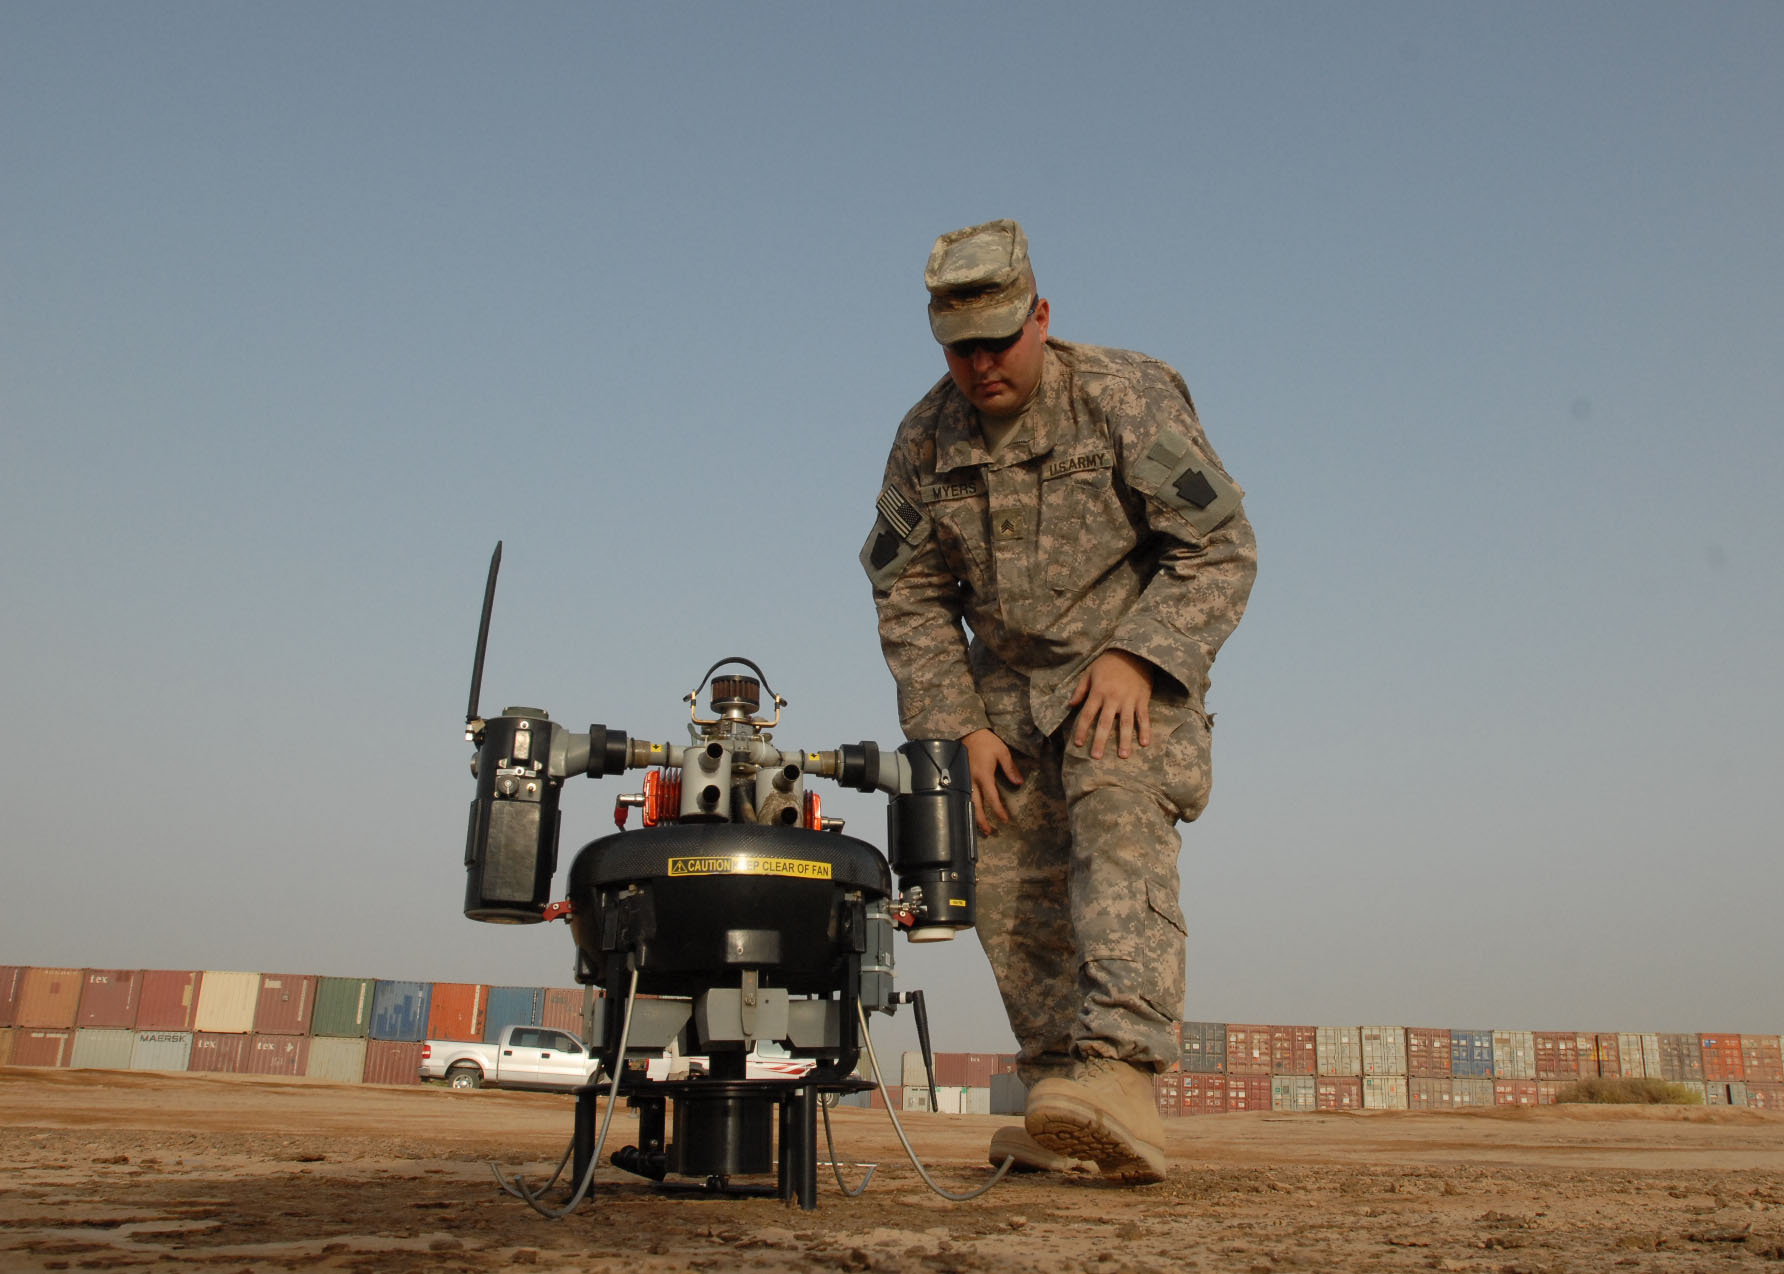
\includegraphics[width=4cm]{img/bitmap_image}
  \caption{Example JPG image.}
  \label{fig:jpg}
\end{figure}


%%% Local Variables: 
%%% mode: latex
%%% TeX-master: "../report"
%%% End: 
% \chapter{A chapter}
\label{sec:a-chapter}

Lorem ipsum dolor sit amet, consectetur adipiscing elit. Sed non risus. Suspendisse lectus tortor, dignissim sit amet, adipiscing nec, ultricies sed, dolor. Cras elementum ultrices diam. Maecenas ligula massa, varius a, semper congue, euismod non, mi. Proin porttitor, orci nec nonummy molestie, enim est eleifend mi, non fermentum diam nisl sit amet erat. Duis semper. Duis arcu massa, scelerisque vitae,  convallis sollicitudin purus. Praesent aliquam, enim at fermentum mollis, ligula massa adipiscing nisl, ac euismod nibh nisl eu lectus. Fusce vulputate sem at sapien. Vivamus leo. Aliquam euismod libero eu enim. Nulla nec felis sed leo placerat imperdiet. Aenean suscipit nulla in justo. Suspendisse cursus rutrum augue. Nulla tincidunt tincidunt mi. Curabitur iaculis, lorem vel rhoncus faucibus, felis magna fermentum augue, et ultricies lacus lorem varius purus. Curabitur eu amet. Encore une citation \cite{Cadambe2008}.

\begin{figure}[htp!]
  \centering
  \setlength\figureheight{7cm}
  \setlength\figurewidth{9cm}
  % This file was created by matlab2tikz v0.2.2.
% Copyright (c) 2008--2012, Nico Schlömer <nico.schloemer@gmail.com>
% All rights reserved.
% 
% 
% 

% defining custom colors
\definecolor{mycolor1}{rgb}{0,0.75,0.75}

\begin{tikzpicture}

\begin{axis}[%
view={0}{90},
width=\figurewidth,
height=\figureheight,
scale only axis,
xmin=2, xmax=4.5,
xlabel={$\eta$},
xmajorgrids,
ymin=0.5, ymax=1,
ylabel={$d_{\text{min}}^2$},
ymajorgrids,
legend cell align=left,
legend style={align=left}]
\addplot [
color=black,
dashed,
mark=asterisk,
mark options={solid}
]
coordinates{
 (2,1)(2.1,1)(2.2,1)(2.3,1)(2.4,1)(2.5,1)(2.6,0.937749781479547)(2.7,0.890900393128398)(2.8,0.864988513955105)(2.9,0.827013168393703)(3,0.811347612650328)(3.1,0.792559278041243)(3.2,0.765840563467819)(3.3,0.749680961469385)(3.4,0.741947149227874)(3.5,0.740609493518419)(3.6,0.732128087463441)(3.7,0.717775843626632)(3.8,0.699687461812158)(3.9,0.685018622769455)(4,0.673439611642851)(4.1,0.664624248264608)(4.2,0.658255928882634)(4.3,0.641702335270489)(4.4,0.608326504614558)(4.5,0.580489221369454) 
};
\addlegendentry{$\alpha\text{ =  0\%}$};

\addplot [
color=black,
dashed,
mark=x,
mark options={solid}
]
coordinates{
 (2,1)(2.1,1)(2.2,1)(2.3,1)(2.4,0.958561324724996)(2.5,0.900812804739278)(2.6,0.859608621629443)(2.7,0.828484932127753)(2.8,0.812298837741994)(2.9,0.778916291864501)(3,0.758500630955482)(3.1,0.748375165853317)(3.2,0.745960208532468)(3.3,0.738441167434538)(3.4,0.715506361296671)(3.5,0.696927131434508)(3.6,0.682276848692725)(3.7,0.671128156410174)(3.8,0.663062783265717)(3.9,0.657680299791254)(4,0.621142740976429)(4.1,0.589786339121755)(4.2,0.564530571776849)(4.3,0.54483432747474)(4.4,0.53008799514765)(4.5,0.519641830384595) 
};
\addlegendentry{$\alpha\text{ = 10\%}$};

\addplot [
color=black,
dashed,
mark=triangle,
mark options={solid}
]
coordinates{
 (2,1)(2.1,1)(2.2,1)(2.3,0.966145915091813)(2.4,0.907589260275562)(2.5,0.862273165052718)(2.6,0.833762738286283)(2.7,0.797262289343802)(2.8,0.774689700869446)(2.9,0.763077871790574)(3,0.759584455148894)(3.1,0.735410358863577)(3.2,0.713220246811223)(3.3,0.695713299974315)(3.4,0.682371019886023)(3.5,0.672682085917092)(3.6,0.6661550402729)(3.7,0.644666127799479)(3.8,0.610083129739041)(3.9,0.582172698611821)(4,0.560333265725228)(4.1,0.543883933286703)(4.2,0.532098369213191)(4.3,0.524242326405)(4.4,0.519608701974017)(4.5,0.517545187250875) 
};
\addlegendentry{$\alpha\text{ = 20\%}$};

\addplot [
color=black,
dashed,
mark=triangle,
mark options={solid,,rotate=180}
]
coordinates{
 (2,1)(2.1,1)(2.2,0.995488894312993)(2.3,0.930050749246739)(2.4,0.882604857341179)(2.5,0.840148695151764)(2.6,0.807621264874927)(2.7,0.787889977099099)(2.8,0.777972678915356)(2.9,0.750463202108443)(3,0.726620292578349)(3.1,0.707917379352703)(3.2,0.693763185722015)(3.3,0.683575144048861)(3.4,0.676795290182409)(3.5,0.663350261880571)(3.6,0.627666127013326)(3.7,0.598755039468926)(3.8,0.575986310488554)(3.9,0.558651995817327)(4,0.546003746104731)(4.1,0.537291509323841)(4.2,0.531798375059385)(4.3,0.528867181690889)(4.4,0.527917002741411)(4.5,0.528450017604181) 
};
\addlegendentry{$\alpha\text{ = 30\%}$};

\addplot [
color=black,
dashed,
mark=o,
mark options={solid}
]
coordinates{
 (2,1)(2.1,1)(2.2,1)(2.3,1)(2.4,1)(2.5,0.995096871086856)(2.6,0.937749790013923)(2.7,0.890900391028178)(2.8,0.864988509535523)(2.9,0.827013167946275)(3,0.811347609462027)(3.1,0.79255927917077)(3.2,0.765840564829299)(3.3,0.749680963181722)(3.4,0.741947149533667)(3.5,0.740609492450166)(3.6,0.732128080624777)(3.7,0.71777584554089)(3.8,0.699687463368726)(3.9,0.681193180471954)(4,0.640212533267028)(4.1,0.617585040920557)(4.2,0.608519007405809)(4.3,0.608298095410932)(4.4,0.608326494076335)(4.5,0.580489212682311) 
};
\addlegendentry{Mazo};

\end{axis}
\end{tikzpicture}%
  \caption{TiKZ curve.}
  \label{fig:tikz-curve}
\end{figure}

\section{Limit Analysis}
Lorem ipsum dolor sit amet, consectetur adipiscing elit. Sed non risus. Suspendisse lectus tortor, dignissim sit amet, adipiscing nec, ultricies sed, dolor. Cras elementum ultrices diam. Maecenas ligula massa, varius a, semper congue, euismod non, mi. Proin porttitor, orci nec nonummy molestie, enim est eleifend mi, non fermentum diam nisl sit amet erat. Duis semper. Duis arcu massa, scelerisque vitae, consequat in, pretium a, enim. Pellentesque congue. Ut in risus volutpat libero pharetra tempor. Cras vestibulum bibendum augue. Praesent egestas leo in pede. Praesent blandit odio eu enim. Pellentesque sed dui ut augue blandit sodales. Vestibulum ante ipsum primis in faucibus orci luctus et ultrices posuere cubilia Curae; Aliquam nibh. Mauris ac mauris sed pede pellentesque fermentum. Maecenas adipiscing ante non diam sodales hendrerit. Ut velit mauris, egestas sed, gravida nec, ornare ut, mi. Aenean ut orci vel massa suscipit pulvinar. Nulla sollicitudin. Fusce varius, ligula non tempus aliquam, nunc turpis ullamcorper nibh, in tempus sapien eros vitae ligula. Pellentesque rhoncus nunc et augue. Integer id felis. Curabitur aliquet pellentesque diam. Integer quis metus vitae elit lobortis egestas. Lorem ipsum dolor sit amet, consectetuer adipiscing elit. Morbi vel erat non mauris convallis vehicula. Nulla et sapien. Integer tortor tellus, aliquam faucibus, convallis id, congue eu, quam. Mauris ullamcorper felis vitae erat. Proin feugiat, augue non elementum posuere, metus purus iaculis lectus, et tristique ligula justo vitae magna. Aliquam convallis sollicitudin purus. Praesent aliquam, enim at fermentum mollis, ligula massa adipiscing nisl, ac euismod nibh nisl eu lectus. Fusce vulputate sem at sapien. Vivamus leo. Aliquam euismod libero eu enim. Nulla nec felis sed leo placerat imperdiet. Aenean suscipit nulla in justo. Suspendisse cursus rutrum augue. Nulla tincidunt tincidunt mi. Curabitur iaculis, lorem vel rhoncus faucibus, felis magna fermentum augue, et ultricies lacus lorem varius purus. Curabitur eu amet.

\subsection{Remarks on the method}
Lorem ipsum dolor sit amet, consectetuer adipiscing elit. Morbi vel erat non mauris convallis vehicula. Nulla et sapien. Integer tortor tellus, aliquam faucibus, convallis id, congue eu, quam. Mauris ullamcorper felis vitae erat. Proin feugiat, augue non elementum posuere, metus purus iaculis lectus, et tristique ligula justo vitae magna. Aliquam convallis sollicitudin purus. Praesent aliquam, enim at fermentum mollis, ligula massa adipiscing nisl, ac euismod nibh nisl eu lectus. Fusce vulputate sem at sapien. Vivamus leo. Aliquam euismod libero eu enim. Nulla nec felis sed leo placerat imperdiet. Aenean suscipit nulla in justo. Suspendisse cursus rutrum augue. Nulla tincidunt tincidunt mi. Curabitur iaculis, lorem vel rhoncus faucibus, felis magna fermentum augue, et ultricies lacus lorem varius purus. Curabitur eu amet.

\begin{align}
H_{m,n,p,q} &= \DPR{\rproto_{p,q}}{\OP{H} \tproto_{m,n}}\\
&= \iint\limits_{\SET{R}^2} S_{\OP{H}}(f,\tau) \DPR{\rproto_{p,q}}{\OP{U}_{f,\tau} \tproto_{m,n}} \ud f \ud \tau.
\end{align}

\section{Numerical verification}
Lorem ipsum dolor sit amet, consectetur adipiscing elit. Sed non risus. Suspendisse lectus tortor, dignissim sit amet, adipiscing nec, ultricies sed, dolor. Cras elementum ultrices diam. Maecenas ligula massa, varius a, semper congue, euismod non, mi. Proin porttitor, orci nec nonummy molestie, enim est eleifend mi, non fermentum diam nisl sit amet erat. Duis semper. Duis arcu massa, scelerisque vitae, consequat in, pretium a, enim. Pellentesque congue. Ut in risus volutpat libero pharetra tempor. Cras vestibulum bibendum augue. Praesent egestas leo in pede. Praesent blandit odio eu enim. Pellentesque sed dui ut augue blandit sodales. Vestibulum ante ipsum primis in faucibus orci luctus et ultrices posuere cubilia Curae; Aliquam nibh. Mauris ac mauris sed pede pellentesque fermentum. Maecenas adipiscing ante non diam sodales hendrerit. Ut velit mauris, egestas sed, gravida nec, ornare ut, mi. Aenean ut orci vel massa suscipit pulvinar. Nulla sollicitudin. Fusce varius, ligula non tempus aliquam, nunc turpis ullamcorper nibh, in tempus sapien eros vitae ligula. Pellentesque rhoncus nunc et augue. Integer id felis. Curabitur aliquet pellentesque diam. Integer quis metus vitae elit lobortis egestas. Lorem ipsum dolor sit amet, consectetuer adipiscing elit. Morbi vel erat non mauris convallis vehicula. Nulla et sapien. Integer tortor tellus, aliquam faucibus, convallis id, congue eu, quam. Mauris ullamcorper felis vitae erat. Proin feugiat, augue non elementum posuere, metus purus iaculis lectus, et tristique ligula justo vitae magna. Aliquam convallis sollicitudin purus. Praesent aliquam, enim at fermentum mollis, ligula massa adipiscing nisl, ac euismod nibh nisl eu lectus. Fusce vulputate sem at sapien. Vivamus leo. Aliquam euismod libero eu enim. Nulla nec felis sed leo placerat imperdiet. Aenean suscipit nulla in justo. Suspendisse cursus rutrum augue. Nulla tincidunt tincidunt mi. Curabitur iaculis, lorem vel rhoncus faucibus, felis magna fermentum augue, et ultricies lacus lorem varius purus. Curabitur eu amet.

%%% Local Variables: 
%%% mode: latex
%%% TeX-master: "report"
%%% End: 
% \chapter*{Conclusion and Outlook}
\addcontentsline{toc}{chapter}{Conclusion}
\markboth{Conclusion}{Conclusion}
\label{sec:conclusion}

    Lorem ipsum dolor sit amet, consectetur adipiscing elit. Sed non risus. Suspendisse lectus tortor, dignissim sit amet, adipiscing nec, ultricies sed, dolor. Cras elementum ultrices diam. Maecenas ligula massa, varius a, semper congue, euismod non, mi. Proin porttitor, orci nec nonummy molestie, enim est eleifend mi, non fermentum diam nisl sit amet erat. Duis semper. Duis arcu massa, scelerisque vitae, consequat in, pretium a, enim. Pellentesque congue. Ut in risus volutpat libero pharetra tempor. Cras vestibulum bibendum augue. Praesent egestas leo in pede. Praesent blandit odio eu enim. Pellentesque sed dui ut augue blandit sodales. Vestibulum ante ipsum primis in faucibus orci luctus et ultrices posuere cubilia Curae; Aliquam nibh. Mauris ac mauris sed pede pellentesque fermentum. Maecenas adipiscing ante non diam sodales hendrerit. Ut velit mauris, egestas sed, gravida nec, ornare ut, mi. Aenean ut orci vel massa suscipit pulvinar. Nulla sollicitudin. Fusce varius, ligula non tempus aliquam, nunc turpis ullamcorper nibh, in tempus sapien eros vitae ligula. Pellentesque rhoncus nunc et augue. Integer id felis. Curabitur aliquet pellentesque diam. Integer quis metus vitae elit lobortis egestas. Lorem ipsum dolor sit amet, consectetuer adipiscing elit. Morbi vel erat non mauris convallis vehicula. Nulla et sapien. Integer tortor tellus, aliquam faucibus, convallis id, congue eu, quam. Mauris ullamcorper felis vitae erat. Proin feugiat, augue non elementum posuere, metus purus iaculis lectus, et tristique ligula justo vitae magna. Aliquam convallis sollicitudin purus. Praesent aliquam, enim at fermentum mollis, ligula massa adipiscing nisl, ac euismod nibh nisl eu lectus. Fusce vulputate sem at sapien. Vivamus leo. Aliquam euismod libero eu enim. Nulla nec felis sed leo placerat imperdiet. Aenean suscipit nulla in justo. Suspendisse cursus rutrum augue. Nulla tincidunt tincidunt mi. Curabitur iaculis, lorem vel rhoncus faucibus, felis magna fermentum augue, et ultricies lacus lorem varius purus. Curabitur eu amet.

%%% Local Variables: 
%%% mode: latex
%%% TeX-master: "report"
%%% End: 



%% Binding Word Spelling Definitions --------------------
%% - when in doubt: check merriam-webster.com (American English!)
%% - headings: use title case, like capitalizemytitle.com
%% - frontend, backend
%% - band plot, DOS plot, band-DOS plot
%% - one-dimensional, three-dimensional
%% - unit cell, supercell
%% - capitalized words:
%%   - proper names
%%     - example: Brillouin zone
%%     - counterexample: density of states
%% - formulas:
%%   - dispersion relation: $E(\mathbf{k})$
%%   - Chemical formula: $\textrm{MoSe}_2$
%% - bullet lists:
%%   - Capitalize complete sentences.
%%   - lowercase sentence fragment
%% ------------------------------------------------------



\chapter{Introduction}
\label{chap:intro}

\section{Problem Statement}
\label{sec:problem-statement}

%% CP: proofread modification v1 of PK Original ======================================== 
One important problem in solid-state physics is the computation of electronic properties of materials, especially crystals. Since the quantum mechanical equations which describe the physics of electrons in solids are usually impossible to solve with analytical methods, numerical codes were developed to solve these equations efficiently on high-performance computers. The project `Fleur' that this project is based on is a highly optimized code that solves the many-body problem based on the DFT (Density functional theory) approach \cite{fleur}.

Fleur is a freely available full potential linearized augmented planewave (FLAPW) code developed by physicists at the Forschungzentrum Jülich. Like any other kind of numerical simulation, DFT simulations produce a significant amount of data that needs to be preprocessed, visualized and analyzed in order to gain physical insight. 

The whole pipeline, from the raw data generated by Fleur through data exploration to comprehensible plots showing selected physical properties of the simulated material, is addressed in this project. 


% %% PK Original ========================================
% Solid State physics deals with the study of large scale properties of solid materials resulting from the atomic scale properties. A solid state physicist can get to know the atomic scale properties from the experiments conducted on the material. Another way to elucidate physical properties is numerical simulation by means of Density Function Theory (DFT). This method is computational Quantum mechanical modeling method to investigate the electronic structure of many body systems of an atom or molecule. Electron density, Intermolecular forces, charge transfer excitations, calculation of band gap among others are properties that are made amenable by DFT simulations.

% Fleur is one such DFT simulation which is developed by physicists at Juelich Forchungzentrum and most importantly its an open source and anyone can access it and use it. Like any other simulation, DFT simulation also outputs a lot of data for a solid state physicist to understand and determine the properties of a cell structure of a molecule through which physical properties of the material can be determined. Fleur is run specifying the cell structure of a molecule and so can be used on any molecule's cell structure and obtain the characteristics of same.

% Generally it is used to find/simulate properties of solids with impurities in cell structure. Fluer outputs the data of DFT simulation. It gives the data of ground state and excited state properties of solids. These data which are raw are generally not accessible directly and have to be processed through steps for any solid state physicist to understand the raw data extracted from Fleur DFT simulation. This becomes the major problem and which is dealt in this project. The goal of this project was to implement a complete data analysis pipeline for this application. The steps include preprocessing followed by data exploration and visualization.


\section{Motivation and Requirements}
\label{sec:motiv-requ}

%% CP: proofread modification v1 of PK Original ========================================
The main project goal was to develop a software product that is able to perform
all necessary steps of postprocessing including visualization in order to make
the Fleur simulation output easily accessible for both solid-state physicists
and non-experts who use Fleur for the first time alike. 

This imposes several requirements on the software:
\begin{itemize}
    \item Physically accurate and meaningful representation of data: The data reduction strategy during the preprocessing must be transparent and physically motivated. Plots should be in a format well known by any physicist.
    \item Easy to use: The tool must not be overloaded with functionalities for very specific problems, but is supposed to be general and usable in an intuitive way without much explanation.
    \item Easy to access: The tool should be able to run in, or from, different environments with no additional setup.
    \item Reasonably fast: The datasets can be large, therefore efficient preprocessing and plotting techniques are necessary.
    \item Easy to extend and maintain: In order to let the software developed in
        the scope of this project keep pace with external improvements and new
        tools, the code should be written in a modular style.
    \item Export feature: Visualization results have to be exportable as PDF or PNG.
\end{itemize}

The central piece of the project from the physics point of view is the `backend', which is a library that reads the simulation data and prepares it for the visualization. In this module, the dimensionality of data gets reduced according to the choice of the user in a physically meaningful way. The preprocessed data is then passed to a `frontend', that visualizes the preprocessed data. To reach a wide range of potential users, the authors decided to develop a graphical user interface (GUI), where parameters relevant to the visualization can be passed interactively. The visualization produced within this interactive tool can then be exported in order to be shared and discussed.

% %% PK Original ========================================
% An API which solves the physicist's problem of understanding the simulation data which transforms raw data to useful data such that it is process and visualizes. This API has to process the output files from fleur directly so that it is easier for physicists to get the data processed without external effort. Having said this, modularization and easy maintainability of code also matters since the format and structure of simulation results keeps varying over the time with the development of simulation code and more data may be collected from simulation.

% This API shouldn't only be solving the physicist's problem but also should be fast enough in terms of computation. As known, using of computer code to get outputs and may cause confusions in using it as computer code and there is always chance of altering the code while using it. So a front end GUI is needed such that a physicist can use the GUI to input the parameters and to output the processed data. As this is used for research purpose and the features such as plots, images and other should be of high quality and resolution such that there is no uncertainty of the results.


\section{Project Steps}
\label{sec:steps}

%% CP: proofread modification v1 of PK Original
%% ========================================
The project was organized into several steps with the supervisors.
\begin{itemize}
\item Understanding the problem: Understand. the physics of the datasets and how
    the data is used in research. This leads to a list of requirements that the
    software has to fulfill in order to be usable in a productive way.
\item Preprocessing: Write a backend that reads raw data and processes it by transforming it into a format that can be visualized in an efficient way. Therefore, the dimensionality of the data needs to be reduced without losing too much physical information.
\item Exploring the data: Investigate possible challenges that might occur during the visualization of the data. (e.g. how to deal with points/datasets covering each other, ...)
\item Visualization: The preprocessed data is visualized in a scatter plot with
    a format well known in the physics community.
\item Frontend: A GUI with intuitive features is developed such that a wide
    range of users can access Fleur output without having to deal with the raw data. 
\item Test the usability of the software using typical Fleur output files. Prove that physical insight can be gained easily using the software.
\item Deployment: Bring the project into a form that can be distributed.
\end{itemize}


% %% PK Original ========================================
% The project steps by step procedure has completed to complete the task of processing and visualization.
% \begin{itemize}
% \item Understanding the problem: Firstly the theory of DFT simulation, Fleur code, band plots, density plots, file format of data and other necessary theory needed are learnt and problem of the project to process the data in different steps is understood.
% \item Pre-Processing: Once problem is clearly understood, first step of project comes to preprocessing the data. Reading the data, sorting the data and storing it sorted which can be used in further stages of implementation.
% \item Exploring the data: From the raw data, not just band plots but many features can be extracted. Finding out the features through exploring the data and trying to understand and extract those features is done.
% \item Visualization: The data which is pre-processed and extracted need to be visualized into plots such that any user with solid state physics background can understand it with an observation.
% \item Front End: A GUI is developed so that its easier in future for any physicist to just run the GUI and get the plots and other visualization instead going through hassle of code and letting a chance of code being disturbed unintentionally
% \item Results and lookup: Getting to know the features extracted, studying it,
%     reporting the same.
% \end{itemize}




%%% Local Variables:
%%% mode: latex
%%% TeX-master: "../"
%%% End:

%  LocalWords:  frontend


\chapter{Theoretical Background}
\label{chap:theory}

%...some introduction scentence depending on intro chapter...

%The visualization pipeline developed in this project is supposed to process data that is produced by the scientific code Fleur \cite{fleur}.

Fleur computes the electronic structure in crystals using the density functional theory approach (DFT), which is one of the state of the art method for this problem. The many-body Schrödinger equation, that can be used to describe electrons in solids, is almost impossible to solve directly, because the storage of the wavefunctions of each of the $N$ electrons in the system at each spatial coordinate exceeds the memory of any currently available computer for even quite small $N$. This motivates the DFT approach, that uses two fundamental theorems to reduce the computational complexity of the many-body problem significantly: The Hohenberg-Kohn theorem \cite{hohenberg-kohn} allows to use the electron density instead of the $N$-electron wavefunctions to uniquely characterize the ground state of a system. With the Kohn-Sham equations \cite{kohn-sham}, the interacting Hamiltonian of the system can be replaced by non-interacting equations with an effective potential. This so-called KS-DFT approach reduces the dimensionality of the problem from $N^3$ to $3$ and trades the interacting Hamiltonian for a set of non-interacting equations that have to be solved self-consistently. In general, the DFT approach is not just limited to computations of electrons in crystals, but is also for example used in chemistry to compute nonperiodic molecules.
% 
The output of a DFT calculation includes various physical quantities, for instance, the three-dimensional spatial electron density, which is the central quantity in DFT calculations. In this project, however, we focus on two quantities that are easy to interpret, already reduced in dimensionality and frequently used in both experimental and theoretical physics.

The band structure $E(\mathbf{k})$ represents the eigenenergies of the eigenfunctions of the Hamiltonian for each crystal momentum $\mathbf{k}$. It is the dispersion relation of electrons in the crystal and relates allowed momenta and energies. In general, $E(\mathbf{k})$ is defined at any point inside the Brillouin zone, which is a special choice of the unit cell in the reciprocal lattice of the crystal. Both, the real space lattice and the reciprocal lattice are shown for a face-centered cubic (fcc) crystal in figure \ref{fcc}. For larger unit cells with fewer symmetries, the Brillouin zone can be much more complicated than in the shown example. In order to reduce the dimensionality of $E(\mathbf{k})$ with $k \in {\rm I\!R}^3$, the dispersion relation is only sampled along a discrete one-dimensional path between high symmetry points in the Brillouin zone. This path still contains most of the relevant physical features.

\begin{figure}[htb!]
    \centering
    \begin{subfigure}{.5\textwidth}
        \centering
        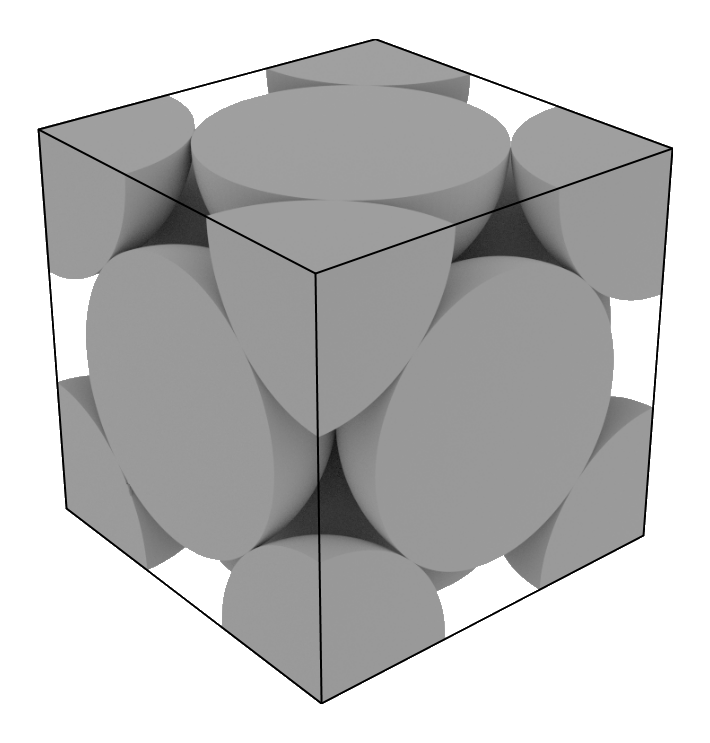
\includegraphics[width=0.5\linewidth]{christian/fcc_real.png}
        \caption{Lattice in real space}
        \label{fig:fcc_real}
    \end{subfigure}% %this '%' is needed for side-by-side figure!
    \begin{subfigure}{.5\textwidth}
        \centering
        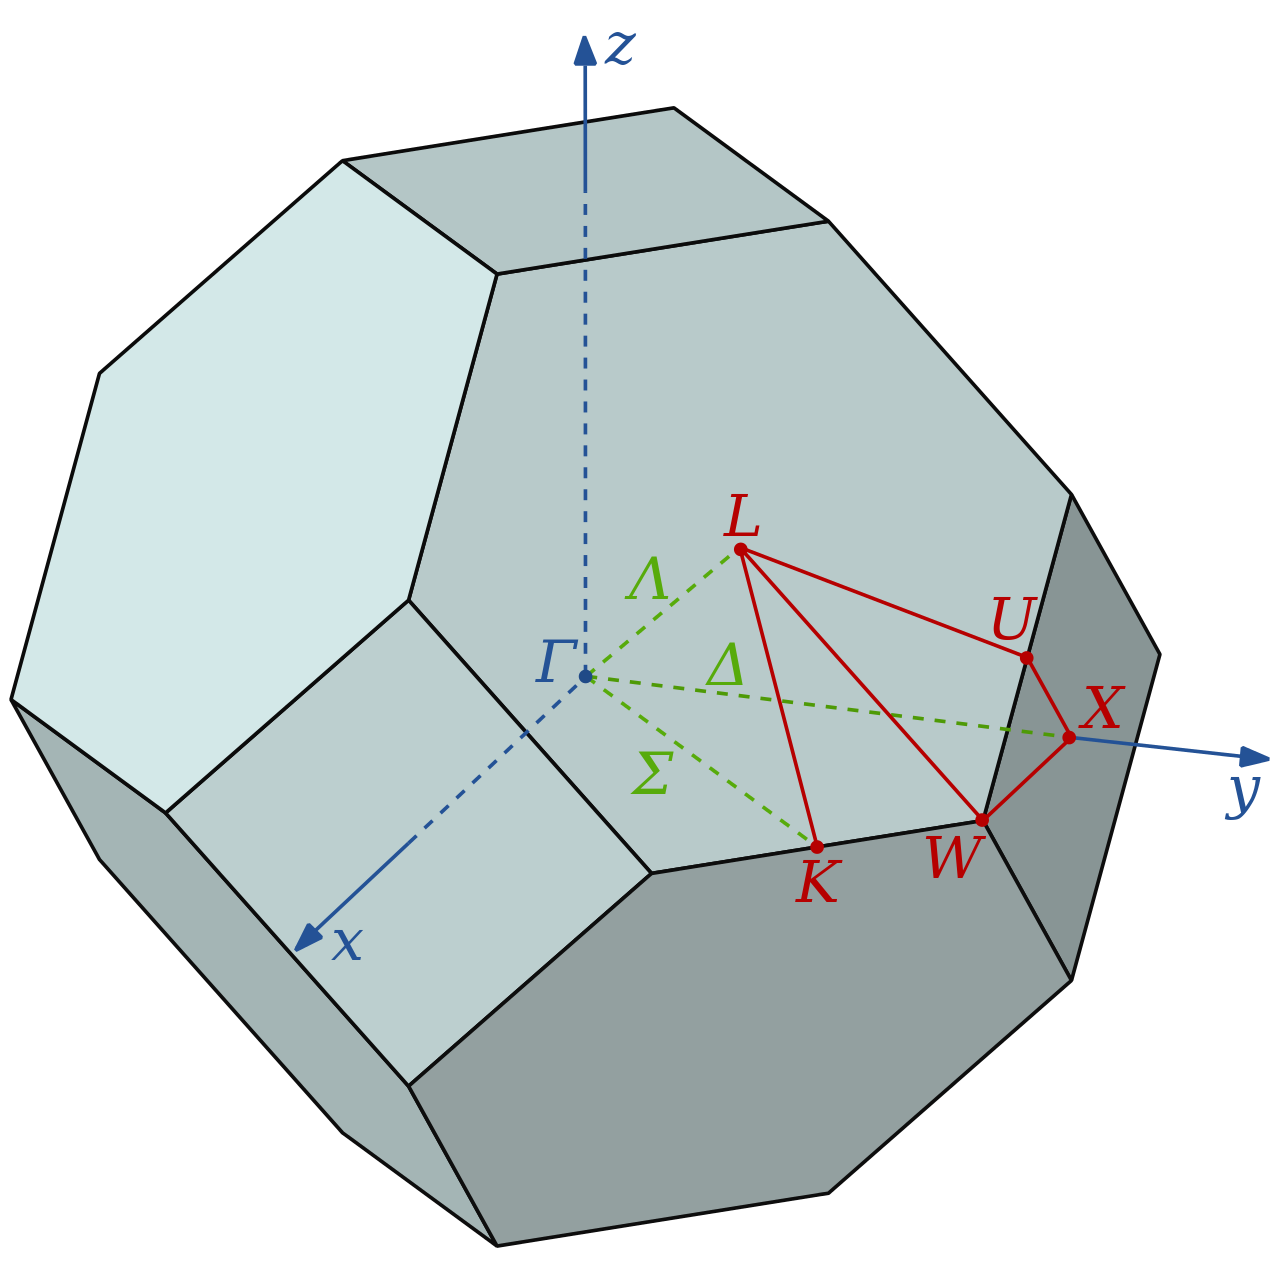
\includegraphics[width=0.5\linewidth]{christian/Brillouin_Zone_(1st,_FCC).png}
        \caption{Brillouin zone}
        \label{fig:fcc_billouin}
    \end{subfigure}
    \caption[Brillouin zone of an fcc lattice]{Brillouin zone of an fcc lattice. The red curve in the reciprocal lattice represents a possible sampling path of $E(\mathbf{k})$ in the reciprocal lattice.}
    \label{fcc}
\end{figure}

The second central quantity in this project is the density of states (DOS)
$D(E)$, which describes the number of states per energy interval that is
independent of the crystal momentum. In this sense, the DOS is also derived from
$E(\mathbf{k})$, but instead of just selecting a subset, the $\mathbf{k}$
dependency is summed out. This sum is performed internally by Fleur, since
$E(\mathbf{k})$ must be known at every grid point in the Brillouin zone. Both complementary quantities together are a common choice for comprehensive visualizations of electronic structure data while still capturing most of the important physics. 

For applications, it is useful to investigate where the contributions to $E(\mathbf{k})$ and $D(E)$ come from. Therefore, the data contains the weights of each basis function of the DFT calculation belonging to the individual atom groups and the orbitals. This means that spatial information about the system can be restored by considering only contributions from certain atom groups. (An atom group contains all atoms that are equivalent with respect to symmetries of the real space lattice.) On the other hand, the projection on the (hydrogen-type) orbitals s, p, d, f encode information about the shape of the wavefunction at each atom. These contributions are stored in the form of relative weights that can be summed to include contributions for multiple groups and orbitals. In case of distinct spins in the crystal, $E(\mathbf{k})$, $D(E)$ and the weights can be different for both spins and are therefore stored individually.



%%% Local Variables:
%%% mode: latex
%%% TeX-master: "../report"
%%% End:


\chapter{Implementation}
\label{chap:implementation}
% logo definitions
\newcommand{\logoFleur}{%
  \begingroup\normalfont
  
\includegraphics[height=1.2\fontcharht\font`\B]{img/logo/fleur.png}%
  \endgroup
}
\newcommand{\logoAiida}{%
  \begingroup\normalfont
  
\includegraphics[height=1.0\fontcharht\font`\B]{img/logo/aiida.png}%
  \endgroup
}
\newcommand{\logoAiidalab}{%
  \begingroup\normalfont
  
\includegraphics[height=1.0\fontcharht\font`\B]{img/logo/aiidalab.png}%
  \endgroup
}
\newcommand{\logoBinder}{%
  \begingroup\normalfont
  
\includegraphics[height=1.2\fontcharht\font`\B]{img/logo/binder.png}%
  \endgroup
}
\newcommand{\logoBokeh}{%
  \begingroup\normalfont
  
\includegraphics[height=1.2\fontcharht\font`\B]{img/logo/bokeh.png}%
  \endgroup
}
\newcommand{\logoDash}{%
  \begingroup\normalfont
  
\includegraphics[height=1.2\fontcharht\font`\B]{img/logo/dash.png}%
  \endgroup
}
\newcommand{\logoDocker}{%
  \begingroup\normalfont
  
\includegraphics[height=1.2\fontcharht\font`\B]{img/logo/docker.png}%
  \endgroup
}
\newcommand{\logoHoloviews}{%
  \begingroup\normalfont
  
\includegraphics[height=1.2\fontcharht\font`\B]{img/logo/holoviews.png}%
  \endgroup
}
\newcommand{\logoHvplot}{%
  \begingroup\normalfont
  
\includegraphics[height=1.2\fontcharht\font`\B]{img/logo/hvplot.png}%
  \endgroup
}
\newcommand{\logoJavascript}{%
  \begingroup\normalfont
  
\includegraphics[height=1.2\fontcharht\font`\B]{img/logo/javascript.png}%
  \endgroup
}
\newcommand{\logoJupyter}{%
  \begingroup\normalfont
  
\includegraphics[height=1.2\fontcharht\font`\B]{img/logo/jupyter.png}%
  \endgroup
}
\newcommand{\logoMatplotlib}{%
  \begingroup\normalfont
  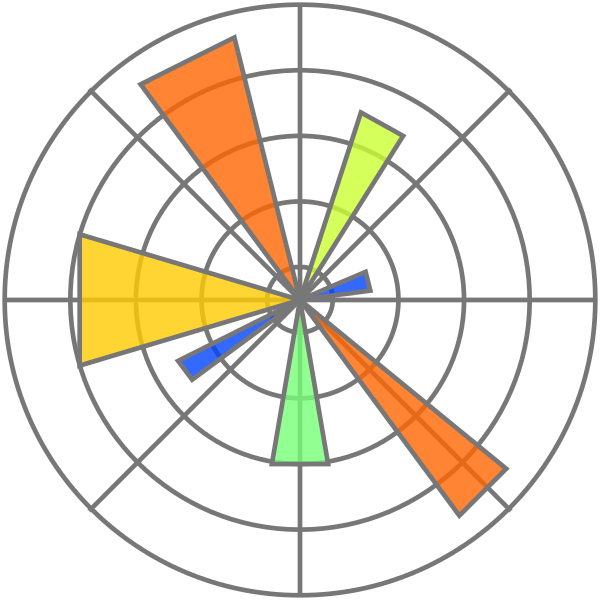
\includegraphics[height=1.2\fontcharht\font`\B]{img/logo/matplotlib.png}%
  \endgroup
}
% \newcommand{\logoMpld3}{%
%   \begingroup\normalfont
%   
\includegraphics[height=1.2\fontcharht\font`\B]{img/logo/mpld3.png}%
%   \endgroup
% }
\newcommand{\logoPanel}{%
  \begingroup\normalfont
  
\includegraphics[height=1.2\fontcharht\font`\B]{img/logo/panel.png}%
  \endgroup
}
\newcommand{\logoParam}{%
  \begingroup\normalfont
  
\includegraphics[height=1.2\fontcharht\font`\B]{img/logo/param.png}%
  \endgroup
}
\newcommand{\logoPlotly}{%
  \begingroup\normalfont
  
\includegraphics[height=1.2\fontcharht\font`\B]{img/logo/plotly.png}%
  \endgroup
}
\newcommand{\logoPython}{%
  \begingroup\normalfont
  
\includegraphics[height=1.2\fontcharht\font`\B]{img/logo/python.png}%
  \endgroup
}
\newcommand{\logoPyviz}{%
  \begingroup\normalfont
  
\includegraphics[height=1.2\fontcharht\font`\B]{img/logo/pyviz.png}%
  \endgroup
}
\newcommand{\logoSeaborn}{%
  \begingroup\normalfont
  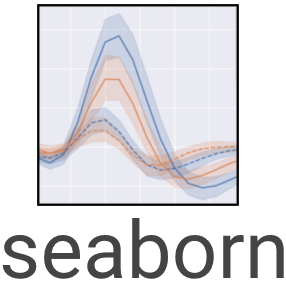
\includegraphics[height=1.2\fontcharht\font`\B]{img/logo/seaborn.png}%
  \endgroup
}

%%% Local Variables:
%%% mode: latex
%%% TeX-master: t
%%% End:


As per the requirements expounded upon in the introduction, the deliverable of
the project should be a finished software product. The software is written in
Python so as to integrate easily with the research group's ongoing software
projects around the Fleur code \cite{fleur}. These are chiefly the group's
materials science tool collection \texttt{masci-tools} \cite{masci-tools} ,
where also this project's code is hosted, and the 'Automated Interactive
Infrastructure and Database for Computational Science' (AiiDA) \cite{aiida}. The
product stakeholders split into frontend users and code developers. In order to
accommodate this, the product is organized into three unidirectionally dependent
subpackages or -modules, see Figure \ref{fig:submodules}.

An important design consideration was to account for unknown use cases. This has
been realized in each submodule by the decoupling of \textbf{interface} and
\textbf{implementation}. The interfaces do not rely on any specific input file
format, visualization method or package, unlike the implementations for a
specific task or \textbf{application}. The word 'application' in this section
denotes the band structure and density of states visualization, and for these,
implementations are provided.

This design choice was also one reason why the product does not reuse any of the
\texttt{masci-tools} routines which partly solve quite similar problems, but
seemed to be too specialized in an cursory code review. For these developers,
one added value of the project product could be to inspire the hopefully easy
integration into a common interface, where the current abstraction level could
serve as a starting point.

%% Bad: jumbles up text
% \begin{wrapfigure}{r}{0.3\textwidth}
%     \centering
% \end{wrapfigure}

%% bad: too near to page side margins
% \begin{figure}[htb!]
%     \centering
%     \begin{subfigure}{.5\textwidth}
%         \centering
%         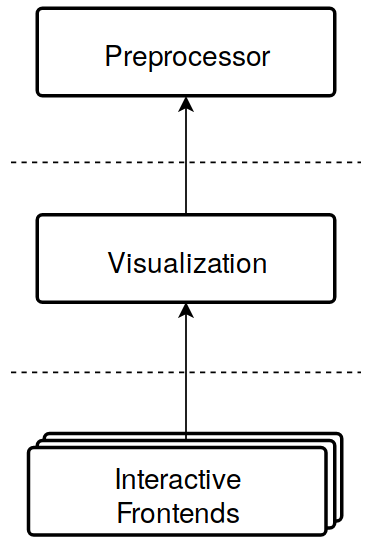
\includegraphics[width=0.5\textwidth]{img/module_design.png}
%         \caption{Submodules}
%         \label{fig:submodules}

%     \end{subfigure}% %this '%' is needed for side-by-side figure!
%     \begin{subfigure}{.7\textwidth}
%         \centering
%         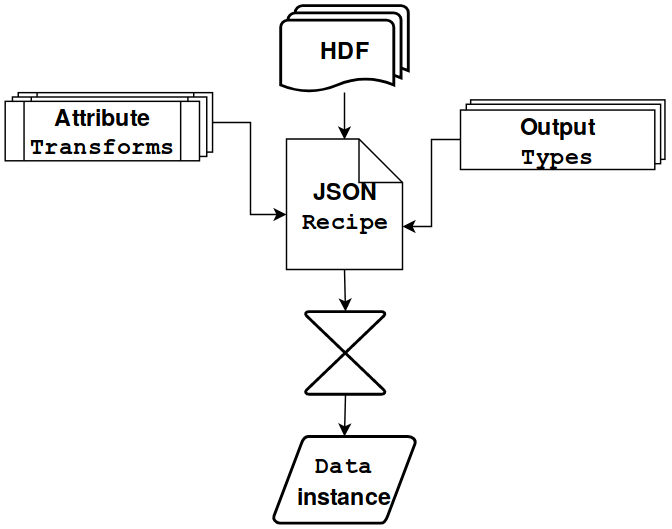
\includegraphics[width=0.7\textwidth]{img/reader_flowchart4.png}
%         \caption{Preprocessor}
%         \label{fig:preprocessor}
%     \end{subfigure}
%     \caption{Module Design.}
%     \label{fig:module-design}
% \end{figure}


\begin{figure}[htb!]
    % Fixed length
    \centering
    \subcaptionbox{Submodules\label{fig:submodules}}{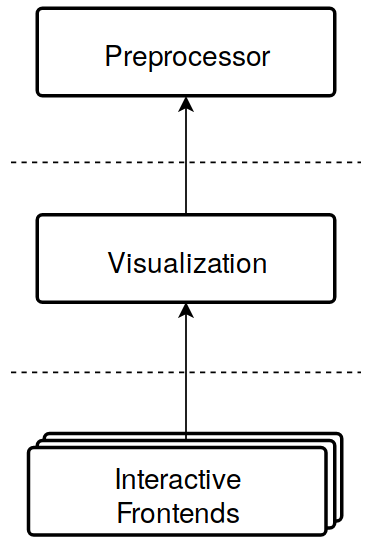
\includegraphics[width=1.6in]{img/module_design.png}}\hspace{5em}%
    \subcaptionbox{Preprocessor\label{fig:preprocessor}}{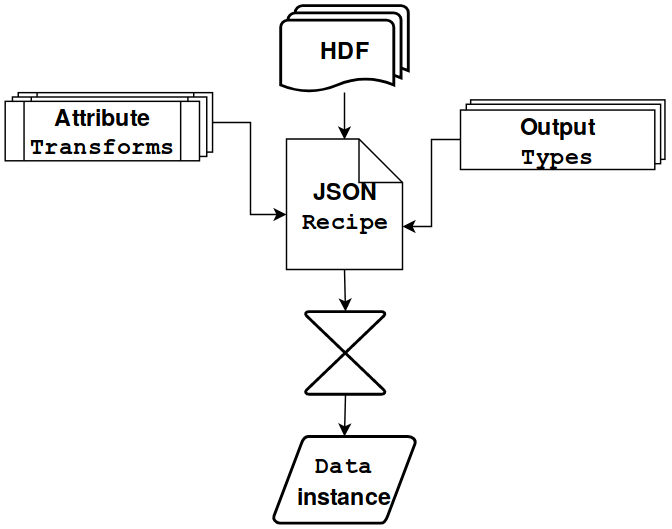
\includegraphics[width=0.5\textwidth]{img/reader_flowchart4.png}}
    \caption{Module Design.}
    \label{fig:module-design}
\end{figure}


\section{HDF Preprocessor Module}
\label{sec:preprocessor-module}

\subsection{Interface}
\label{sec:preprocessor-interface}

This is the 'backend' of the tool. It is basically a file reader for the input
data, for example a Fleur simulation output. Supported formats are the
Hierarchical Data Format (HDF) \cite{hdf} for the band structure, and a simple
Fleur-specific comma-separated values (CSV) format for the density of states
(DOS).

The HDF format is basically a binary flexible container for all kinds of common
binary and text file formats, each of which constitutes a \texttt{Dataset}
inside the HDF file. The format supports metadata annotation and high-throughput
input/output (I/O). As a consequence, it is considered by some developers in
some application domains relying on numerical simulation codes, to be one
possible base for the establishment of common domain-specific rich data exchange
standards in order to increase code interoperability. These developers are in
the process of extending their codes' I/O capabilities towards that end.
However, HDF's flexibility comes at the price of a relatively complex Application
Programming Interface (API) as the keyhole for all operations.

The preprocessor module tries to hide that complexity by offering the
\texttt{Recipes} interface, see Figure \ref{fig:preprocessor}. A specific
application \texttt{Recipe} is a dictionary that aims to describe a complete
\href{https://en.wikipedia.org/wiki/Extract,_transform,_load}{Extract-Transform-Load}
(ETL) pipeline for one specific application. The 'extract' is the reading of a
dataset from HDF, the 'transform' a sequence of once-through functions applied
to the the dataset, and the 'load' the aggregation of all transformed datasets
into one runtime object that has all the methods for operations on the data that
are going to be used later on in the intended application.

The 'transform' and 'output' type methods are defined in hierarchical
\texttt{Transform} and \texttt{Output\_Type} classes, which sort them from
general to application-specific applicability. This structure is built using
Python's \texttt{AbstractBaseClass} (\texttt{ABC}) interface and multiple
inheritance. The advantages of the 'Recipes approach' are:
\begin{itemize}
\item All ETL processes for one application are collected in one simple list
    (the recipe), not locked in different code locations with conflicting
    contexts. In this list, entries can be sorted in any manner, e.g.
    alphabetical for perusal. Thus a recipe also serves as a concise
    documentation of how an application-domain HDF format expects to be handled.
\item Recipes are de/serializable (can be read from and saved to disk) and thus be
    created and manipulated by code.
\item The ETL processes declared in this way can be easily reused across
    applications. A recipe can combine different output types into a new type.
\end{itemize}

The feature that enables this flexibility is \textbf{type introspection}: the
preprocessor processes the datasets listed in the recipe in the order of their
mutual dependencies as found in the used transform and output methods. When all
transformed datasets have been added to the object, all specified output types
are searched and all their methods and attributes added. Thus the output
object's type is defined at runtime, when the preprocessing is finished.

% \begin{figure}[htb!]
%     \centering
%     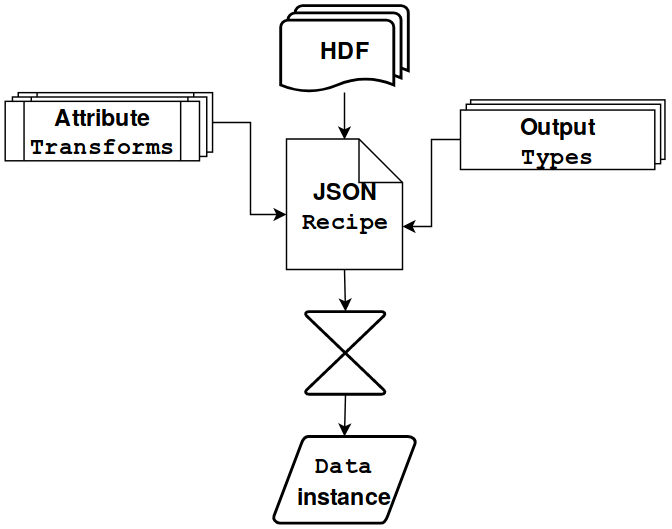
\includegraphics[width=0.6\textwidth]{img/reader_flowchart4.png}
%     \caption{The preprocessor module.}
%     \label{fig:preprocessor}
% \end{figure}

% \lstinputlisting[
% language=python,
% style=code,
% linerange=101-106
% captionpos=t,
% caption={Recipe \texttt{FleurBands} excerpt: dataset \texttt{BravaisMatrix}},
% label=recipe
% ]{listings/recipes.py}


\subsection{Implementation for Band Structure Visualization}
\label{sec:preprocessor-implementation}

\textbf{TODO} describe how bandstructure data is preprocessed for visualization
including user selections AND optimizations

The frontend has to draw three kinds of plots: a 3D atom plot of the unit cell
or supercell, and a combined band structure and DOS plot sharing the same
vertical energy axis. If no DOS data is present, the DOS plot will be omitted.
All three plots are controlled by one set of widgets for varying the parameters.
In the current implementation, the data for the first two plots come from a HDF
file, while the data for DOS plot come from CSV files.

The band structure plot is a scatter plot and plots discrete \(E(\mathbf{k})\) data
from the simulation. It first needs the \(k\)-path (where \(|\mathbf{k}|=k\)) for
the horizontal axis. The preprocessor, having received the recipe
\texttt{FleurBands}, computes it from the \(k\)-points in the HDF in a
transform. Next, the plot needs the eigenergies for every point on the
\(k\)-path, labeled by the band index \(\nu\), and its associated \(l\)-like
charge \(n_{s,k,\nu,g,l}\). It is fivedimensional, and represents the
contribution of spin \(s\), point \(k\) point on \(k\)-path, band \(\nu\), atom
group \(g\), and character or orbital \(l\) (here: only s,p,d,f) to the specific
eigenergy. In order to visualize this, resolves the processed data into the
like-named output type \texttt{FleurBands}. This type has a data filter method.
The respective \texttt{BandPlot} type calls this filter with a user selection of
subsets of all \((s,k,\nu,g,l)\). The method then computes the according
\textbf{effective weight} shown in Equation \ref{eq:effective-weight}. This is
used for the dot size of each \(E(k)\) in the plot. Before rendering, the
plotter normalizes the energies to the Fermi Energy.

\begin{align}
  W^{\text{eff}}_{s,k,\nu} = \left( \frac{\sum\limits_{\substack{g \in \text{groups} \\ l \in \text{characters}}} n_{s,k,\nu,g,l}\, N_g}{\sum\limits_{\substack{g \in \text{all groups} \\ l \in \text{all characters}}} n_{s,k,\nu,g,l}\, N_g} \right) \left(W_{s,k,\nu}^{\text{unf}}\right)^\alpha
\label{eq:effective-weight}
\end{align}

\(N_g\) denotes the number of atoms in a group. \(W_{s,k,\nu}^{\text{unf}}\) is
the unfolding weight and \(\alpha\) its exponent. The effect of unfolding is
illustrated in Figure \ref{fig:unfolding} for a toy example of a monatomic
chain, with a two-atom supercell of size \(a'\) representing \(\alpha=0\) and a
one-atom unit cell of size \(a\) representing \(\alpha=1\). A use-case is
discussed in the Application Chapter \ref{chap:applications}.

\begin{figure}[htb!]
    \centering
    
\includegraphics[width=0.6\linewidth]{fig/unfolding.png}
    \caption[Band Unfolding]{Band Unfolding: Example for a simple monatomic
      chain \cite{hoffmann1987chemistry}.}
    \label{fig:unfolding}
\end{figure}

Even for small band structures, the filter has to access on the order \(10^7\)
individual data points for every selection change. Optimizations were introduced
which included: a cutoff skipping effective weights too small,use of optimized
Numpy functions like \texttt{np.tensor}, data buffering, and array reshaping.
Together, these achieve a speedup of approximately \(10^2\) in plotting speed.
Thanks to that, the tool remains usable even when input data is in the \(10^2\)
MB range.

\section{Visualization Module \& Interactive Graphical Frontends}
\label{sec:visualization-module}

\textbf{TODO} Frontends: combine into one subsection when finished. usage will
be in user manual next section.

\subsection{Visualization Module}
\label{sec:visualization-interface}

The Python visualization landscape abounds with a rapidly evolving plethora of
plotting libraries for different application contexts and technology stacks
\cite{python-viz-landscape}. Thus the project's visualization module first
design objective was to account for that by decoupling from specific library
use, and modularizing applications. This structure again is built using Python's
\texttt{AbstractBaseClass} (\texttt{ABC}) interface and multiple inheritance.
Each application is represented by an abstract base class that contains the
common plotting method signatures. Each plotting library is represented by an
abstract base class that contains library-specifics. An implementation inherits
both from one library base class and one or more application base classes. See
Fig. \ref{fig:visualization-module} for an impression. Thus switching the
library in a frontend should require minimal adjustment, and a new application
can be build using existing ones.

The second design objective was for the plotting methods to to hide all
interactions with the actual plotting library used under the hood, while the
method arguments only relate to the preprocessed data being plotted. Thus
different frontend implementations only all call one common method for one
specific plot and receive the identical visualization with identical interactive
behavior.

\begin{figure}[htb!]
    \centering
    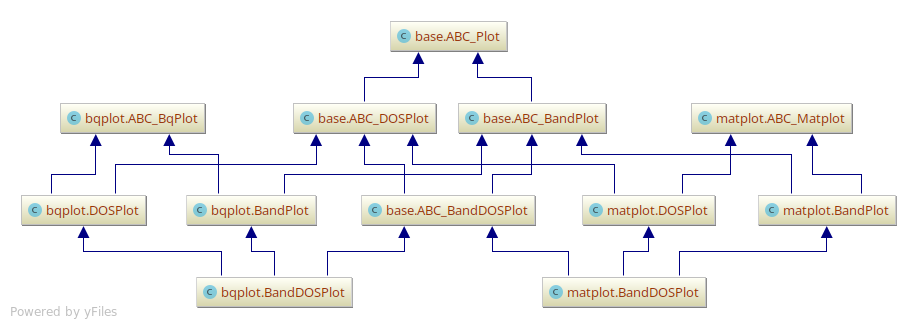
\includegraphics[width=1.0\linewidth]{img/pycharm_uml/matplot.png}
    \caption[Visualization Module Design]{Visualization Module Design: Example
      Structure for two applications \texttt{BandPlot} and \texttt{DOSPlot}, and
      two plotting libraries \texttt{matplotlib} and \texttt{bqplot}.}
    \label{fig:visualization-module}
\end{figure}

\subsection{Desktop Frontend}
\label{sec:desktop-frontend}

A Desktop Frontend is always a helping had for the physicists to just run it on the computer when one wants to go through the plots of the raw data that is already in computer. 
Since the reading of HDF files and preprocessing of the data is done using Python, it is decided that it would be better to use python for front end development. Considering various packages for front end in python such as PyQt, Tkinter and other packages available for Desktop frontend, the conventional tkinter is selected based on the maintainability of the code. It is a package where every button can be designed and can be assigned to function.
Functions like label, button, checkbutton, listbox, canvas for plots, tab for viewing each plot in different tab are used to make a simple Desktop front end. It is simple to use with limited options of what any physicist needed and also easy to convert it into a executable software and run in any system without any installation.

\subsection{Web Frontend}
\label{sec:web-frontend}

As Web Frontends increasingly replace traditional Desktop Frontends in the
modern software environment \cite{web-vs-desktop}, so Python-based Frontends and
visualizations are increasingly moving towards the browser. There, GUIs with
interactive visualizations are often called \textbf{Dashboards}. In the project
context, a survey was undertaken in order to choose the most suitable technology
stack. The full survey is documented in \cite{jw-notes}. The requirements for
the solution stack, added to those in the introduction, were as follows:

\begin{enumerate}
\item \textbf{openness}: relies solely on Open-Source-Software (OSS) with
    licensing suitable for academic use, sports a stable release cycle, developer
    base and documentation,
\item \textbf{dashboarding}: features graphical control elements (widgets) that
    interact with InfoVis\footnote{InfoVis libraries: visualizations of
      information in arbitrary spaces, not necessarily the three-dimensional
      physical world. Example: matplotlib. SciVis libraries: visualizing
      physically situated data. Example: VTK \cite{python-viz-2018}.} plotting
    libraries,
\item \textbf{deployment}: ideally works like any web service, i.e. only a
    modern web browser is required to use it,
\item \textbf{maintenance}: requires only Python and no Web Development
    knowledge like e.g. Javascript, with respect to the product stakeholders.
\end{enumerate}

The last point implies a client-server model where the dashboard app is hosted
by a remote service. This model requires a communication framework and protocol
between the Python interpreter running on the server and the JavaScript
interpreter running in the client browser. As per requirement number two, unlike
a generic Python web framework like e.g. \href{http://flask.pocoo.org/}{Flask},
the framework should take care of that communication by itself. Four major
frameworks were identified which fulfill the first three requirements:
\href{https://jupyter.org/}{Project Jupyter}, \href{http://pyviz.org/}{PyViz},
\href{https://bokeh.pydata.org/en/latest/}{Bokeh}, and
\href{https://plot.ly/products/dash/}{Dash by Plotly}. The last two only
partially fulfilled the last requirement, so they were discarded. PyViz is the
newest contender among the four. Its expressed goal is to untangle the Python
visualization jungle by providing one high-level API that ties together all
major Python InfoVis libraries and data formats, including dashboarding. That
ambitious goal comes at the price of sacrificing support for 3D plotting
\cite{pyviz-faq}, which was needed in this project for the atoms plot. So PyViz
had to be discarded.

That left Project Jupyter. By now, it's widget library \texttt{ipywidgets} is
integrated to work with a wide variety of popular plotting libraries. However,
Jupyter only partially fulfills the third requirement -- a Jupyter notebook
(app) cannot, by itself, be published (deployed) as a stand-alone website
outside a live Jupyter environment \cite{python-viz-2018}:

\begin{quote}
    [...] ``However, despite their web-based interactivity, the ipywidgets-based
    libraries (ipyleaflet, pythreejs, ipyvolume, bqplot) are difficult to deploy
    as public-facing apps because the Jupyter protocol allows arbitrary code
    execution'' [...].
\end{quote}

To avoid requiring users to setup a working Jupyter environment on their
machine, the go-to solution for this problem is to setup a
\href{https://jupyter.org/hub}{JupyterHub} multi-user server. This still
requires users to register an account there. Fortunately though, the intended
users are contributors to the AiiDA project, and so should have access to the
JupyterHub-based \href{ https://aiidalab.materialscloud.org/}{AiiDaLab} service
where the app can be registered. Details on this procedure and alternative
hosting solutions can be found in the developer Section
\vref{for-developers}.


%%% Local Variables:
%%% mode: latex
%%% TeX-master: "../report"
%%% End:

%  LocalWords:  subpackages submodule


\chapter{Manual}
\label{cha:manual}

The project code and documentation is hosted on the \texttt{masci-tools}
repository \cite{masci-tools} under the branch
\href{https://github.com/JuDFTteam/masci-tools/tree/studentproject18ws}{\texttt{studentproject18ws}}.
All of the project code resides in the folders \texttt{binder} (for the web
frontend demo) and \texttt{studentproject18w} (all code and documentation). The
\texttt{README.md} in the latter folder serves as the manual. Therefore, the
remaining part of this chapter is a \TeX{}-ified version of that
\texttt{README.md}, commit
\href{https://github.com/JuDFTteam/masci-tools/tree/7f4d21e1508f0cb5cc0b228ec0802755617c4ed3
}{\texttt{7f4d21e1508f0cb5cc0b228ec0802755617c4ed3}}.

\vspace{3em}
\hdashrule{\textwidth}{2pt}{2pt}
%% BEGIN TEXIFIED README ========================================
%% 
%% Command to TeXify README.md from masci-tools/studentproject18ws:
%% pandoc -s README.md -o README.tex
%% 
%% Manual changes needed after TeXification:
%% - update commit SHA-1 above!
%% - remove badges on top (binder badge, ...)
%% - 'try it out here on': convert to ordinary link without binder badge image
%% - figure -> figure*
%% - texttt{long} -> path{long} (enables linebreak)
%% - '\textgreater{}' -> '>'
%% - replace code sections 'Tok' with lstlisting:
%% \begin{lstlisting}[language=python, style=code]
%% \end{lstlisting}
%% 

\href{https://www.aices.rwth-aachen.de/en/academics/masters-program-simulation-sciences}{SiScLab
2018} Student Project \textbf{Analysis Tool for Materials
  Design}. Written in Python3.

Authors: \href{https://github.com/Irratzo}{Johannes Wasmer},
\href{https://github.com/ChristianPartmann}{Christian Partmann}, and
\href{https://github.com/PraneethKatta}{Praneeth Katta}.

\section{Overview}\label{overview}

This subfolder \texttt{studentproject18ws} is currently a largely
independent side-project accompanying the main module
\texttt{masci-tools}. It was created in a student project at \href{http://www.fz-juelich.de/pgi/pgi-1/EN/Home/home_node.html}{FZJ PGI-1}, and consists
of three submodules:

\begin{itemize}
    \tightlist
\item
    preprocessor: a general
    \href{https://www.hdfgroup.org/solutions/hdf5/}{HDF5} reader interface, and
    one implementation for band structure simulation output of the DFT code \href{http://www.judft.de}{Fleur}
\item visualization: a plotting interface, and one implementation for
    \href{http://www.judft.de}{Fleur} band structure and density of states (DOS)
    plots
\item
    frontends: a desktop GUI and a web dashboard (Tk and Jupyter) for
    interactive Fleur band-DOS plots.
\end{itemize}

A more thorough description and example use cases can be found in the
project \href{./doc/report.pdf}{report} and
\href{./doc/presentation.pdf}{presentation}.

\begin{figure*}
    \centering
    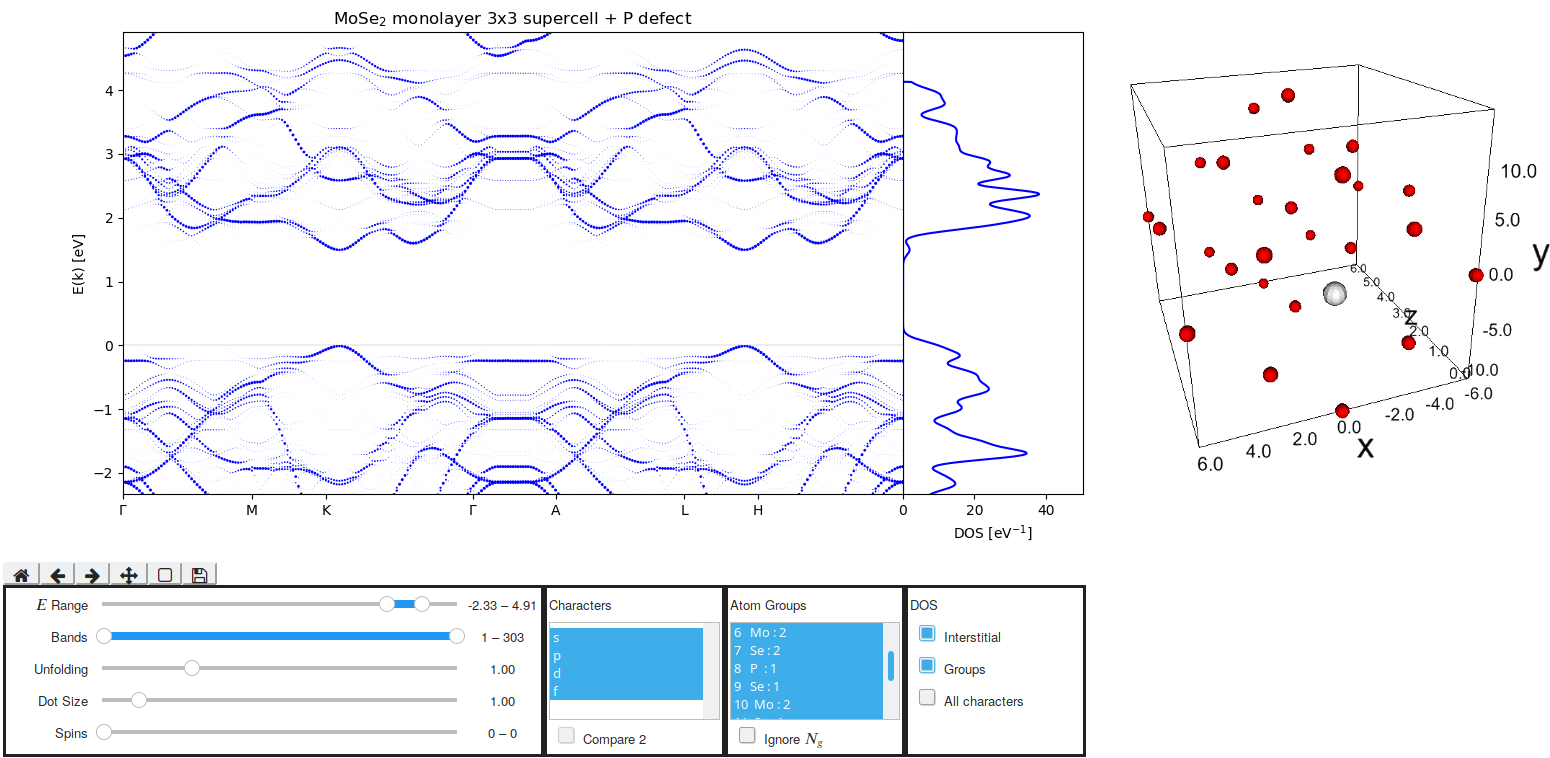
\includegraphics{./readme/web_frontend.png}
\end{figure*}

\section{For Frontend Users}\label{for-frontend-users}

\subsection{General Remarks}\label{general-remarks}

These remarks apply to all frontends.

Though the desktop and web frontend are functionally identical, there
might be small differences in how the controls are used and how they are
labeled.

\subsubsection{File Input}\label{file-input}

The frontends currently expect band structure data in the HDF output format of
\href{http://www.judft.de}{Fleur}. The DOS data is expected
to be in the CSV output format of \href{http://www.judft.de}{Fleur}, one file
per spin. If no DOS files are supplied, the frontend will just draw a band
structure plot (band plot) and omit the adjoined DOS plot. Thus, in the
following band-DOS plot stands for both kinds of plot.

\subsection{Desktop Frontend}\label{desktop-frontend}

\subsubsection{Access}\label{access}

A windows executable file (.exe) is made by packing all the required packages
into the file. Any modern PC running on windows can run the frontend without any
installation process. You don't need Python or specific packages installed.

The executable for Windows (or other operating systems) can be obtained from the developers upon request.

\subsubsection{Usage}\label{usage}

The desktop-based GUI is easy to use. Running the .exe file will open up the
frontend with all packages loaded. The GUI consists of three tab windows. In the
first tab window, absolute paths to the input data files must be entered in this
order: HDF and (optional) DOS file for spin `0' and `1'. Tab 2 shows the
band-DOS plot, and Tab 3 the 3D atoms plot. After loading the files, the controls
must be initialized. Finally, clicking the 'Update' button produces the plots.


Controls for all three plots: 

\begin{itemize}\tightlist
\item \textbf{Update, SaveButton}: redraw the plots with the new selection / save the the plot as a PDF.
\item \textbf{Atom Groups}: redraw only for the selected symmetry groups.
\end{itemize}

Controls for the band and DOS plots:

\begin{itemize}\tightlist
\item \textbf{Ymin, Ymax}: limit the energy range.
\item \textbf{BandMin, BandMax}: limit the band range.
\item \textbf{Character}: likewise for the characters (orbitals) 'S','P','D','F'.
\item \textbf{Spin}: draw bands and DOS for one or both spins.
\end{itemize}

Controls for the band plot only:

\begin{itemize}\tightlist
\item \textbf{Marker Size}: set the marker size of the dots (eigenenergies).
\item \textbf{Exponential weight}: The unfolding exponent for supercell calculations (see \href{./doc/report.pdf}{report}). Value 0.0 means no unfolding. If the calculation is done with a unit cell, this control has no effect.
\item \textbf{Compare 2 Characters}: show the respective contribution of the two selected characters to each eigenergy using a sequential (2) colormap. Disabled if other than two characters are selected.
\item \textbf{Ignore Atom Group}: set the contribution of each group to be equal
    instead of to the number of atoms per group.
\end{itemize}

Controls for the DOS plot only:

\begin{itemize}\tightlist
\item \textbf{Select groups}: include selected atom groups in the DOS
\item \textbf{Interstitial}: include the interstitial in the DOS
\item \textbf{All characters}: include all characters in the DOS regardless of character selection. In the DOS CSV file, different input data is used (a summed column).
\end{itemize}

\subsubsection{Troubleshooting}\label{troubleshooting}

If the band plot is not visible:

\begin{itemize}
    \tightlist
\item
    Click update two to three times.
\item
    Check if the three input files (if any) are belonging to the same
    Fleur calculation and selected appropriately.
\item
    Check if at least one Atom Group, one Character, one Spin is selected.
\item
    Check if Ymin is less than Ymax and similarly BandMin is less than
    BandMax such that software is able to plot.
\end{itemize}

If the DOS plot is not visible:

\begin{itemize}
    \tightlist
\item Make sure either Select Groups or Interstitial is selected.
\end{itemize}

If the problem persists, try restarting the GUI. If that fails, please open an
issue to contact the developers.

\subsection{Web Frontend}\label{web-frontend}

\subsubsection{Access}\label{access}

The web frontend is a Jupyter Dashboard. It is in experimental state (no
fileupload yet). You can try it out
\href{https://mybinder.org/v2/gh/JuDFTteam/masci-tools/studentproject18ws?filepath=studentproject18w\%2Ffrontend\%2Fjupyter\%2Fdemo\%2Fbinder_demo.ipynb}{here
  on Binder}. You can also run it locally (see developer section). If you have an
\href{https://aiidalab.materialscloud.org/hub/login}{AiiDaLab account}: the
dashboard is planned to be published as an app there.

\subsubsection{Usage}\label{usage-1}

Using the Dashboard should be self-explanatory to the domain user. Some
tips:

\begin{itemize}
    \tightlist
\item If the plot window is not on startup or gets stuck, reload/rerun once.
\item Plot updates are instantaneous.
\item Empty selections are impossible.
\item Only shows controls for data that is present in the input.
\item Multi-selection boxes: use ctrl or shift to select multiple items. 
\item Slider values can also be typed into the adjoining text box.
\item Try out the zoom and pan tools below the plot, they're useful.
\end{itemize}

\section{For Developers}\label{for-developers}

\subsection{Installation}\label{installation-1}

Clone this repo (branch). Then create a virtual environment for the project.

With conda (recommended): -
\href{https://www.anaconda.com/download}{Install Anaconda (3
  recommended)} - Install the environment \texttt{masci-stupro} with the
necessary and recommended dependencies:

\begin{lstlisting}[language=bash, style=code]
conda create -f environment.yml
source activate masci-stupro
\end{lstlisting}

With virtualenv (untested):

\begin{lstlisting}[language=bash, style=code]
virtualenv masci-stupro
source masci-stupro/bin/activate
pip install -r requirements_pip.txt # install requirements
\end{lstlisting}

\subsection{Programmatic use}\label{using-the-backend}

Though \texttt{masci-tools} is (planned to be) availabe via PyPI, there is
currently no plan to integrate \texttt{studentproject18ws}. If you want to use
it in your code, use it in an IDE, or append the path to your
\texttt{sys.path}:

\begin{lstlisting}[language=bash, style=code]
import sys
if path_repo not in sys.path:
    sys.path.append(path_repo)
    
# now import works
from studentproject18w.hdf.reader import Reader
# ...
\end{lstlisting}

In this example, a Fleur HDF file is preprocessed using the Recipe
\texttt{FleurBands}. The resulting output \texttt{data} with the
extracted and transformed HDF datasets and attached load methods
(Extract-Transform-Load) is then passed to a plotter, alongside some DOS
CSV files for a bandstructure plot using \texttt{matplotlib} as backend
library.

\begin{lstlisting}[language=python, style=code]
from studentproject18w.hdf.reader import Reader
from studentproject18w.hdf.recipes import Recipes
from studentproject18w.plot.matplot import BandDOSPlot
import matplotlib.pyplot as plt

data = None
reader = Reader(filepath=filepath_hdf)
with reader as h5file:
    data = reader.read(recipe=Recipes.FleurBands)
    #
    # Note:
    # Inside the with statement (context manager),
    # all data attributes that are type h5py Dataset are available
    # (on-disk access). When the statement is left, the HDF5 file 
    # gets closed and the datasets are closed.
    #
    # Use data outside the with-statement (in-memory access: all 
    # HDF5 datasets converted to numpy ndarrays):
    data.move_datasets_to_memory()

plotter = BandDOSPlot(plt, data, filepaths_dos)
(fig, ax_bands, ax_dos) = plter.setup_figure()

data_selection = some_selection_process()
plotter.plot_bandDOS(*data_selection)
plt.show()
\end{lstlisting}

\subsection{Try Out the Web Frontend
  Locally}\label{try-out-web-frontend-locally}

The demo notebook with the dashboard is
\path{studentproject18w/frontend/jupyter/demo/demo.ipynb}.

\subsubsection{If Using Jupyter
  Notebook}\label{if-using-jupyter-notebook}

On Windows, omit keyword \texttt{source}.

\begin{lstlisting}[language=bash, style=code]
source activate masci-stupro
cd mypath/masci-tools/studentproject18ws/
jupyter-notebook .
# if Home is not set to this dir, try this instead:
# /home/you/anaconda3/envs/myenv/bin/python /home/you/anaconda3/envs/myenv/bin/jupyter-notebook .
\end{lstlisting}

\subsubsection{If using Jupyter Lab}\label{if-using-jupyter-lab}

Additional installation step needed:

\begin{lstlisting}[language=bash, style=code]
source activate masci-stupro
jupyter labextension install @jupyter-widgets/jupyterlab-manager jupyter-matplotlib ipyvolume
cd mypath/masci-tools/studentproject18ws/
jupyter-lab
\end{lstlisting}

\subsection{Frontend Deployment}\label{frontend-deployment}

\subsubsection{Desktop Frontend}\label{desktop-frontend-1}

To create executables for different operating systems, use
\href{https://www.pyinstaller.org/}{PyInstaller}. The target file is
\texttt{frontend/tkinter/gui.py}.

\begin{lstlisting}[language=bash, style=code]
source activate masci-stupro
conda install -c conda-forge pyinstaller
# if not using conda: pip install pyInstaller
cd mypath/masci-tools/studentproject18ws/
pyinstaller --onefile frontend/tkinter/gui.py
\end{lstlisting}

\subsubsection{Web Frontend}\label{web-frontend-1}

The web frontend is currently a single Jupyter notebook. In order to
publish it as a usable standalone app, additional work has to be done.

\begin{itemize}
    \tightlist
\item
    Create \texttt{frontend/jupyter/Dashboard.py} and
    put code of
    \href{./frontend/jupyter/demo/demo_backend.ipynb}{demo\_backend.ipynb}
    notebook inside it. This will become the widget. Use 
    \href{https://github.com/aiidalab/aiidalab-widgets-base/blob/master/aiidalab_widgets_base/structures.py}{aiidalab-widgets-base
      > StructureUploadWidget} as a template. Create
    \texttt{frontend/jupyter/Dashboard.ipynb} notebook. This will become the app. Use
    \href{https://github.com/aiidalab/aiidalab-widgets-base/blob/master/structures.ipynb}{StructureUploadWidget
      demo notebook} as a template.
\item
    Add \href{https://pypi.org/project/fileupload/}{fileupload} buttons (for
    HDF, DOS) to widget
    (again, like in StructureUploadWidget. See
    \href{./frontend/jupyter/demo/binder_fileupload_test.ipynb}{binder\_fileupload\_test.ipynb}
    notebook for a demo that works with binder.)
\item
    Now the web frontend should work on Binder.
\item
    For publishing the app on \href{https://aiidalab.materialscloud.org}{AiiDA Lab}, it has to be registered in
    the
    \href{https://github.com/aiidalab/aiidalab-registry}{aiidalab-registry}.

    \begin{itemize}
        \tightlist
    \item
        Create a skeleton using the
        \href{https://github.com/aiidalab/aiidalab-app-cutter}{aiidalab-app-cutter}.
    \item
        The project code is in Python3, but aiidalab requires Python2. So
        the code has to first be backported by hand using the \texttt{future}
        package. If this takes too long, maybe try the tool
        \href{https://pypi.org/project/3to2/}{3to2}.
    \item
        Use the simplest app in the registry,
        \href{https://github.com/aiidalab/aiidalab-units}{aiidalab-units} as
        a template. Adapt code.
    \item
        Try it out first in the
        \href{https://www.materialscloud.org/work/quantum-mobile}{Quantum
          Mobile Virtual Machine}, which has aiidalab installed and
        configured. Else try it in a virtual environment with
        \href{https://pypi.org/project/aiidalab/}{aiidalab} installed from
        PyPI.
    \item
        Register the app.
    \end{itemize}
\end{itemize}

Note: other publishing options besides Binder and AiiDALab are listed
\href{https://github.com/markusschanta/awesome-jupyter}{here}. For
instance, \href{http://colab.research.google.com/}{Google Colaboratory}
is a free notebook hosting service that allows environment creation and file upload.

\subsection{Extending the code}\label{extending-the-code}

\subsubsection{Use Case: HDF format that includes DOS data}
\label{sec:use-case:-hdf}


The Fleur output HDF format is expected to change and incorporate more
data. In turn, this project's code has to be extended as well. The
procedure is outlined for a an example use case: the incorporation of
DOS data into the band structure HDF (thus eliminating the need for
separate DOS CSV files). The instructions show how to extend the
preprocessor, the visualization and frontend submodules to that
scenario.

\begin{itemize}
    \tightlist
\item
    Add a new output type to \texttt{hdf/output\_types}, say
    \texttt{FleurBandDOS}. Let it inherit from output type
    \texttt{FleurBands}. If you want an output type just for the DOS as
    well, add a type \texttt{FleurDOS} and let \texttt{FleurBandDOS}
    inherit it.
\item
    Add a new recipe to \texttt{hdf/recipes} e.g. \texttt{FleurBandDOS}.
    Copy unchanged things from recipe \texttt{FleurBands}.
\item
    If needed, add new transforms to \texttt{hdf/input\_transforms}.
    Adhere to the transform function standard there. If there are mutual
    dependencies, add them to the list in the top of the file.
\item
    Add a DOS data selection method to the output type
    \texttt{FleurBands}. The \texttt{DOSPlot} in \texttt{plot/base} types
    will need those to plot the DOS plot. Simply adapt from the function
    in \texttt{dos/reader} for the DOS CSV files, adopt the identical
    signature.
\item
    In the \texttt{DOSPlot} types in submodule \texttt{plot}, add a switch
    to the constructor that can distinguish the three cases (bands,
    bands+CSV DOS, bands+HDF DOS). Use the switch in the \texttt{plotDOS}
    methods, and for the case bands+HDF DOS, call your new
    \texttt{FleurBandDOS} function.
\end{itemize}

\subsubsection{Extending the Visualization
  (Plots)}\label{extending-the-visualization-plots}

\begin{itemize}
    \tightlist
\item
    In addition to the inheritance scheme based on Python
    \texttt{AbstractBaseClass} (ABC) detailed in the
    \href{./doc/report.pdf}{report}, the \texttt{Plot} types in
    \texttt{plot} have an additional facility that helps to keep the
    appearance of different frontends synchronized: each type has an
    attribute \texttt{icdv} of type
    \texttt{InteractiveControlDisplayValues}. This is an ABC with the same
    inheritance as the application Plot types. For every plot control
    argument that an application type's Plot type exposes in it's methods'
    signatures, this attribute describes the parameters of the
    accompanying control widget in the frontend (text label, default
    values, value ranges, and so on). In the current code, only the web
    frontend uses this facility, so the labels in the desktop frontend
    differ slightly.\\
\item
    It is worth pointing out that unlike other languages, Python does not
    enforce implemented abstract methods to have the same method
    signature. However, when a new implementation for a different plotting
    library/backend is added, it is recommended to adopt the
    \texttt{abstractmethod} signature. That way, changing the backend in a
    use case only requires to change the import.
\end{itemize}

\subsection{Open Issues}
\label{sec:open-issues}

\begin{itemize}
\item Running the frontends in a debugger or with a counter reveals: on a plot
    selection change or update, the plot seems to be redrawn not once but
    several times. The cause could not be found so far.
\item In the desktop frontend, the update button has to be clicked several times.
\item In the web frontend, on startup, the plot is only visible after two loads/cell runs.   
\end{itemize}


%% FINISH TEXIFIED MANUAL ========================================
\hdashrule{\textwidth}{2pt}{2pt}






%% =========================================================
%%% Manuals Chapter OLD VERSION ============================
%% =========================================================
% \section{Frontends User Manual}
% \label{sec:user-manual}

% \subsection{System Requirements \& Installation}
% \label{sec:system-requirements}

% The Desktop Frontend is distributed as an executable file. 

% \subsection{Input Data Formats}
% \label{sec:input-data-formats}

% \subsection{GUI Usage}
% \label{sec:gui-usage}

% The Desktop and Web Frontend are functionally identical and use the same
% graphical descriptors. Thus these points hold true for both alike.

% Instead of dragging the sliders, values can be typed into their adjoining value
% displays as well.

% \textbf{TODO}: web frontend: binder or colab link

% \subsection{Troubleshooting}
% \label{sec:troubleshooting}


% \section{Developer Manual}
% \label{sec:developer-manual}

% At the time of this report, the package is written in Python 3. It is hosted on
% the \texttt{masci-tools} repository \cite{masci-tools} under the branch
% \href{https://github.com/JuDFTteam/masci-tools/tree/studentproject18ws}{\texttt{studentproject18ws}}.
% All of the project code resides in the folders \texttt{binder} (for the Web
% Frontend; see below) and \texttt{studentproject18w} (all code and
% documentation). The \texttt{README.md} contains the same installation
% instructions listed here.

% \subsection{Creating the project virtual environment}
% \label{sec:creat-proj-virt}

% \begin{lstlisting}[language=bash, style=code]
% # if using conda (recommended)
% conda create -f environment.yml
% source activate 

% # if using pip (untested)

% \end{lstlisting}

% \subsection{Creating Desktop Frontend Executables}
% \label{sec:creat-deskt-front}



% \subsection{Extending the Preprocessor}
% \label{sec:extend-prepr}

% \subsection{Extending the Visualization \& Frontends}
% \label{sec:extend-visu-}

% \textbf{TODO:} publish on aiidalab 

% \textbf{TODO:} hosting alternatives
% \begin{itemize}
% \item binder with example
% \item google colab (see jupy wiki or jupy awesome) \cite{jupyter-awesome}
% \item voila?
% \end{itemize}







%%% Local Variables:
%%% mode: latex
%%% TeX-master: "../report"
%%% End:

\chapter{Applications}
\label{chap:applications}


To illustrate the use of the graphical user interface, two different physical
applications are shown in the desktop and the web frontend, respectively. From
the physics point of view, the example in the desktop version focuses more on the
density of states and the visualization of spin contributions, while the dataset
in web frontend focuses on the band structure $E(\mathbf{k})$ and the visualization
of defect states in supercells.

\section{Web Frontend: $\textrm{MoSe}_2$ Crystal}

\begin{wrapfigure}{r}{0.4\textwidth} % placed up here cause below would appear
                                % in next section. and in PDF appears next to
                                % matching text.
    \centering
    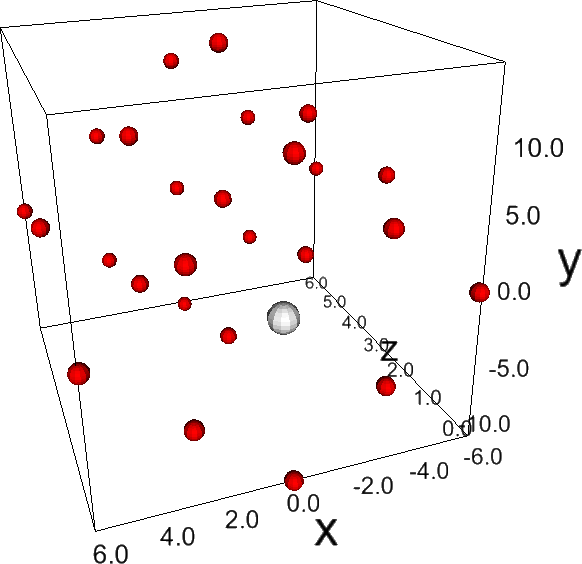
\includegraphics[width=0.38\textwidth]{christian/screen4_atomplot_defect.png}
    \caption[Atom Plot of a $\textrm{MoSe}_2$ monolayer]{Atom Plot of a $MoSe_2$ monolayer with the defect atom selected in
      the web frontend}
    \label{fig:modules}
\end{wrapfigure}

Figure \ref{example1} shows the visualization of a band structure calculation of a 3 dimensional Molybdenum diselenide ($\textrm{MoSe}_2$ bulk) crystal using the default settings of the GUI. Even with the default settings the band structure plots clearly indicate, that $\textrm{MoSe}_2$ is a semiconductor, since there are no states at the Fermi level. Because the minimum of the conduction band is located at an other $k$ as the maximum of the valence band, the plot shows that $\textrm{MoSe}_2$ has an indirect band gap. This indicates that for the transition with the smallest energy difference between valence and the conduction band, both, energy and momentum have to change.

\begin{figure}[htb!]
    \centering
    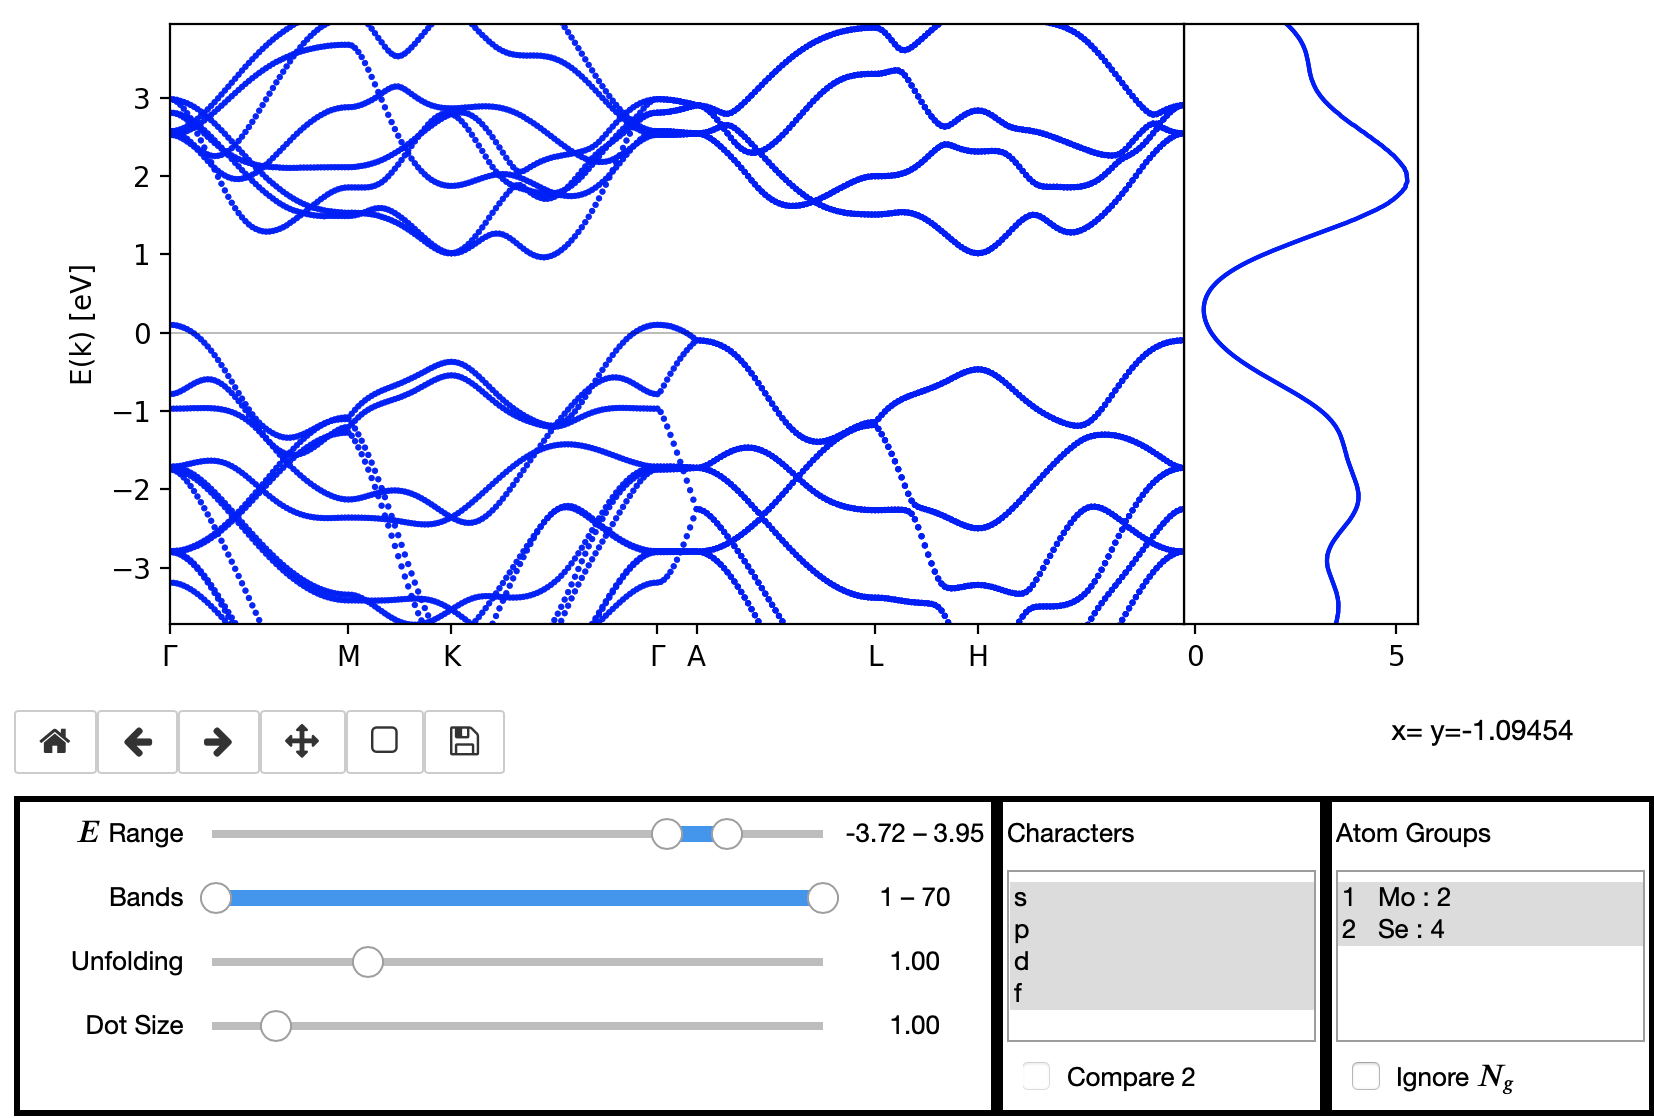
\includegraphics[width=0.7\linewidth]{christian/screen1.png}
    \caption[Bandstructure of a $\textrm{MoSe}_2$ crystal]{Bandstructure of a $\textrm{MoSe}_2$ crystal using the default settings of the web frontend}
    \label{example1}
\end{figure}

In contrast to the 3 dimensional extended $\textrm{MoSe}_2$ crystal, a $\textrm{MoSe}_2$ monolayer (see Fig. \ref{example2}) has a direct band gap but is still a semiconductor. Furthermore, the $\textrm{MoSe}_2$ monolayer has a defect atom in every 9th unit cell and the DFT computation is therefore done in a $3 \times 3$ supercell to restore periodicity. This is the reason for the much greater number of states in the band structure plot. 

\begin{figure}[htb!]
    \centering
    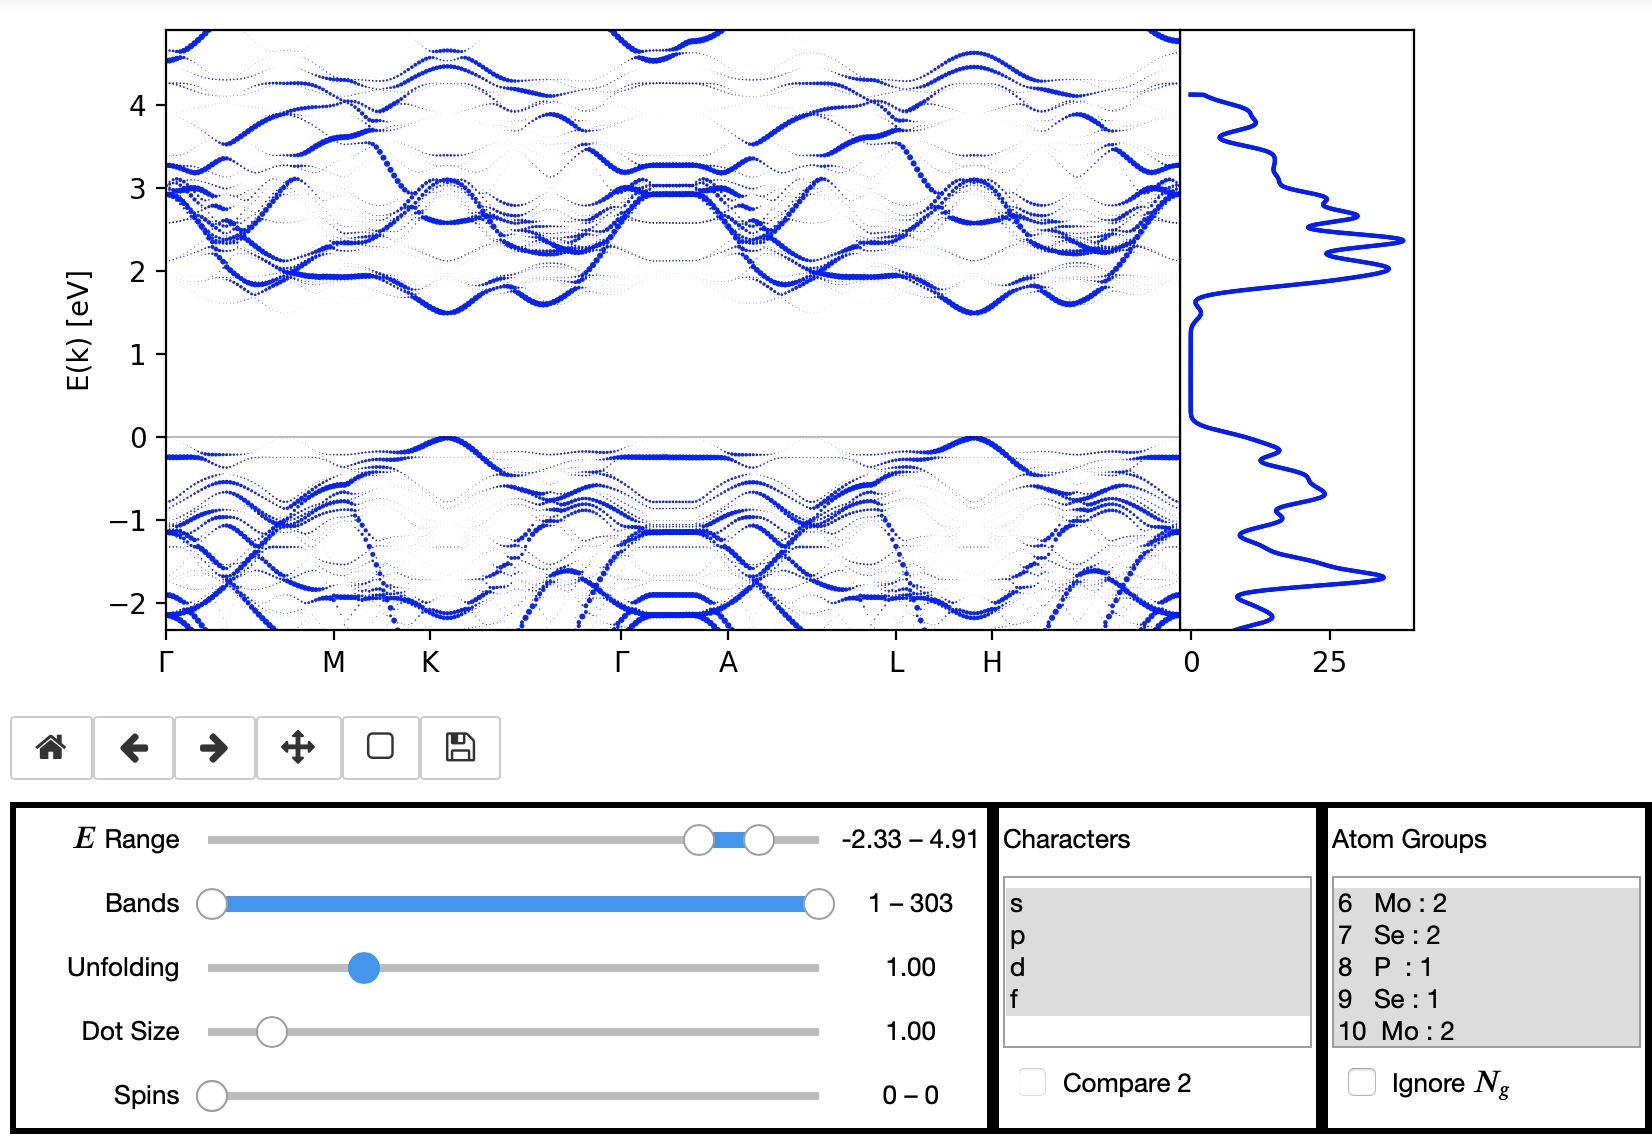
\includegraphics[width=0.7\linewidth]{christian/screen2.png}
    \caption[Bandstructure of a $\textrm{MoSe}_2$ monolayer]{Bandstructure of a $\textrm{MoSe}_2$ monolayer using the default settings of the web frontend}
    \label{example2}
\end{figure}

Since the Brillouin zone of the supercell is smaller than the Brillouin zone of the same crystal without the defect, the supercell Brillouin zone is unfolded to the same size as the Brillouin zone of the unperturbed lattice. To account for the fact that the defect is only present in every 9th cell and its relative importance for the spectrum is therefore degraded, an unfolding weight is introduced to visualize the relative importance of bands in the unfolded Brillouin zone. By default, the unfolding weight is used by our visualization tool, but it can gradually be turned off in order to highlight the impact of defect states. This is shown in figure \ref{example3}. To even better visualize the defect state, it would also be possible to select the atom group belonging the defect atoms only. In this example, the analysis with reduced band unfolding shows, that there are many more direct band gaps origination from the defect state.


\begin{figure}[htb!]
    \centering
    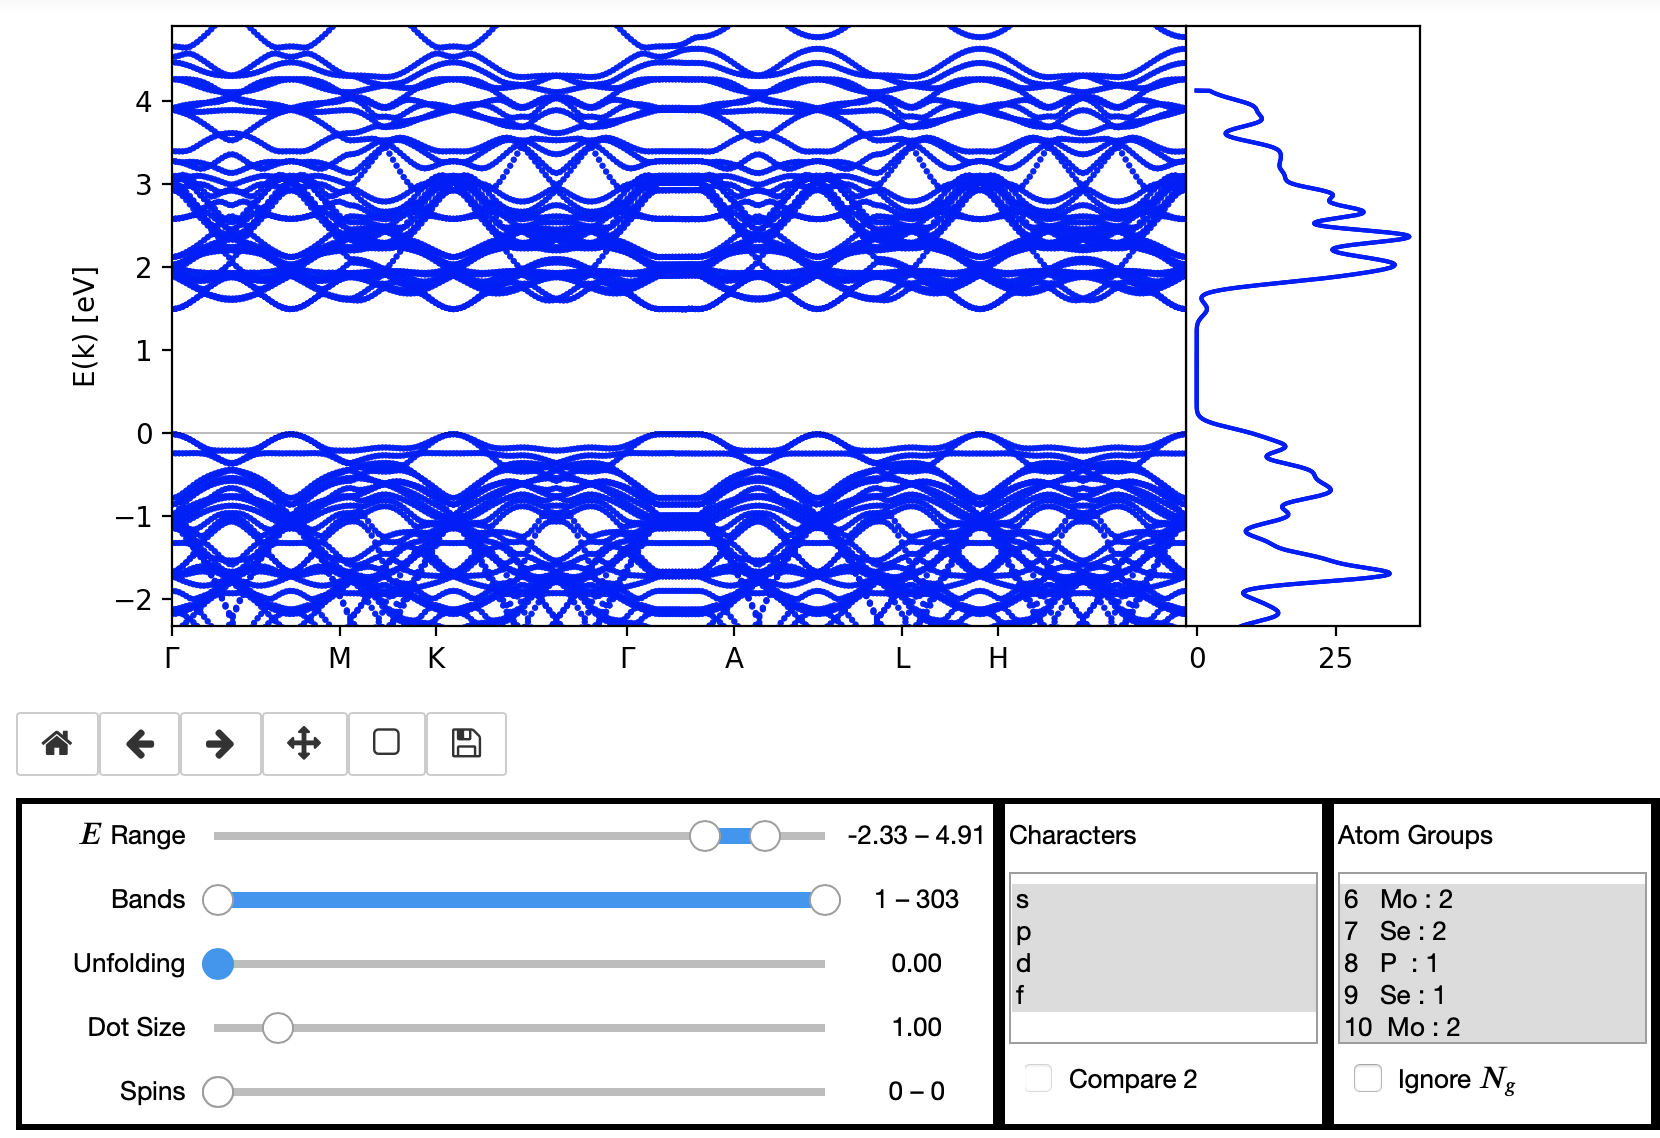
\includegraphics[width=0.7\linewidth]{christian/screen3.png}
    \caption{Bandstructure of a $MoSe_2$ monolayer without unfolding weights}
    \label{example3}
\end{figure}


\section{Desktop Frontend: $\textrm{Co}$ Crystal}

Figure  \textbf{TODO} shows the visualization of a band structure calculation of a 3 dimensional Co crystal with settings of dual spin, one atom group(since it is the only crystal in the cell structure) with all characters and whole band selected with exponent being at $0.0$. We can see in the figure that band plot of any spin intersecting with the Fermi energy level. This means that many electrons excite to valance band which is a characteristic of a conductor. Hence the Co Crystal can be considered and concluded as conductor material.

One more physical property of Co crystal can be determined by considering and reading the density of state(DOS) files and plotting the density of state along with the band plots. In the figure \textbf{TODO}, on the right one can see the Density of states of both the spins. If the area covered under the density is considered, it is clear that under the Fermi energy, electrons of one spin covers more area than other spin in the density of states plot. This means there are more electrons with positive spin under the Fermi energy. This is the character exhibited by the Ferro magnetic substance, so it be considered and concluded that this Co crystal is a Ferro magnetic.

There are two properties which are concluded by observing the band-dos plot but depending on the material and band-dos plot many properties can be extracted and concluded.


\section{Derived physical Quantities: Differentiation}
% bänder isonlieren schwierig....fleur update--> label der E eigenvlas

%$m^{*}$ and $v_{G}(\mathbf{k})$


The kind of datasets handled in the scope of the project did not lend themselves
readily to applications of automatic differentiation techniques. Nevertheless,
it is possible to derive meaningful physical quantities from the band structure
using numerical differentiation techniques.

The effective mass $m^{*}$ represents the mass, that an electron appears to have due to the inter-atomic forces in the crystal. At every $\mathbf{k}_0$, where $E(\mathbf{k})$ has a local extremum, $E(\mathbf{k})$ can be expanded in a Taylor series with a vanishing first order term $E(\mathbf{k}) = E_0 + \frac{\partial E(\mathbf{k})}{\partial \mathbf{k}} \cdot (\mathbf{k}-\mathbf{k}_0)^2$. Comparing this to the dispersion relation of a free electron $E(\mathbf{k})_{free} = \frac{\hbar^2 \mathbf{k}^2}{2 m_e}$ motivates the general definition 

\begin{equation}
    m^{*}_{k_i,k_j} = \hbar^2  \left(\frac{\partial^2E(\mathbf{k})}{\partial k_i \partial k_j}\right)^{-1}
\end{equation}

Since $\frac{\partial^2E(\mathbf{k})}{\partial \mathbf{k}_i \partial \mathbf{k}_j}$ depends on the direction of the partial derivatives, $m^{*}_{k_i,k_j}$ is a tensor. Because the band structure files only contain a discrete sampled path in the Brillouin zone, only the derivatives that correspond to the direction from one high-symmetry point to the next can be computed. We are only interested in the diagonal terms of $m^{*}\big|_{i,j}$.

%maybe something about the directional dependency --> m is tensor...


A second potentially interesting quantity is the group velocity $v_{G}(\mathbf{k})$ associated to each band. The group velocity $v_{G}(\mathbf{k})$ at the Fermi energy $E = E_F$ is called Fermi velocity.

\begin{equation}
    v_{G}(\mathbf{k})_{k_i} = \frac{1}{\hbar}\frac{\partial E(\mathbf{k})}{\partial \mathbf{k_i}}
\end{equation}


\subsection{Differentiation}

Since the k-mesh in DFT calculations is potentially very sparse, low order finite difference schemes are not expected to work well. Alternatively, one way to exploit all data points efficiently is to use fast Fourier transform methods, which are equivalent to the derivation of a truncated Fourier series. This method is expected be well-suited for the problem since the graph of the band structure $(k, E(|k|))$ with $k \in \{-\Gamma,..., H,..., \Gamma\}$ is periodic, where $\Gamma$ and $H$ are arbitrary representatives of the high symmetry points. This periodicity in the reciprocal space is a direct consequence of the periodicity of the crystal.

In Fourier space, spatial derivatives transform into multiplications, which can easily be shown by partial integration.

\begin{equation}
    f^{(n)}(x) = \mathcal{F}^{-1}\left((ik)^n\mathcal{F}(f(x))\right)
\end{equation}
 
To test the FFT differentiation method, a band was selected that did not have intersections with other bands within the interval between two high symmetry points and a stationary point at the high symmetry points. Then a resolution study was done to investigate the impact of the number of points within the interval.

The comparison between the FFT and a first-order central difference approximation of the second derivative (FD) is shown in Fig. \ref{num_diff}, where different k-mesh resolutions are compared to a derivative that is almost fully converged. The comparison indicates that for small N, the error of the FFT method is significantly smaller than the error of the FD derivative. This is especially striking in the vicinity of the high symmetry points, where the error of the differentiation is required to be small in order to get good approximations for $m^{*}$, which is only meaningful close to the high symmetry points.


\begin{figure}[htb!]
    \centering
    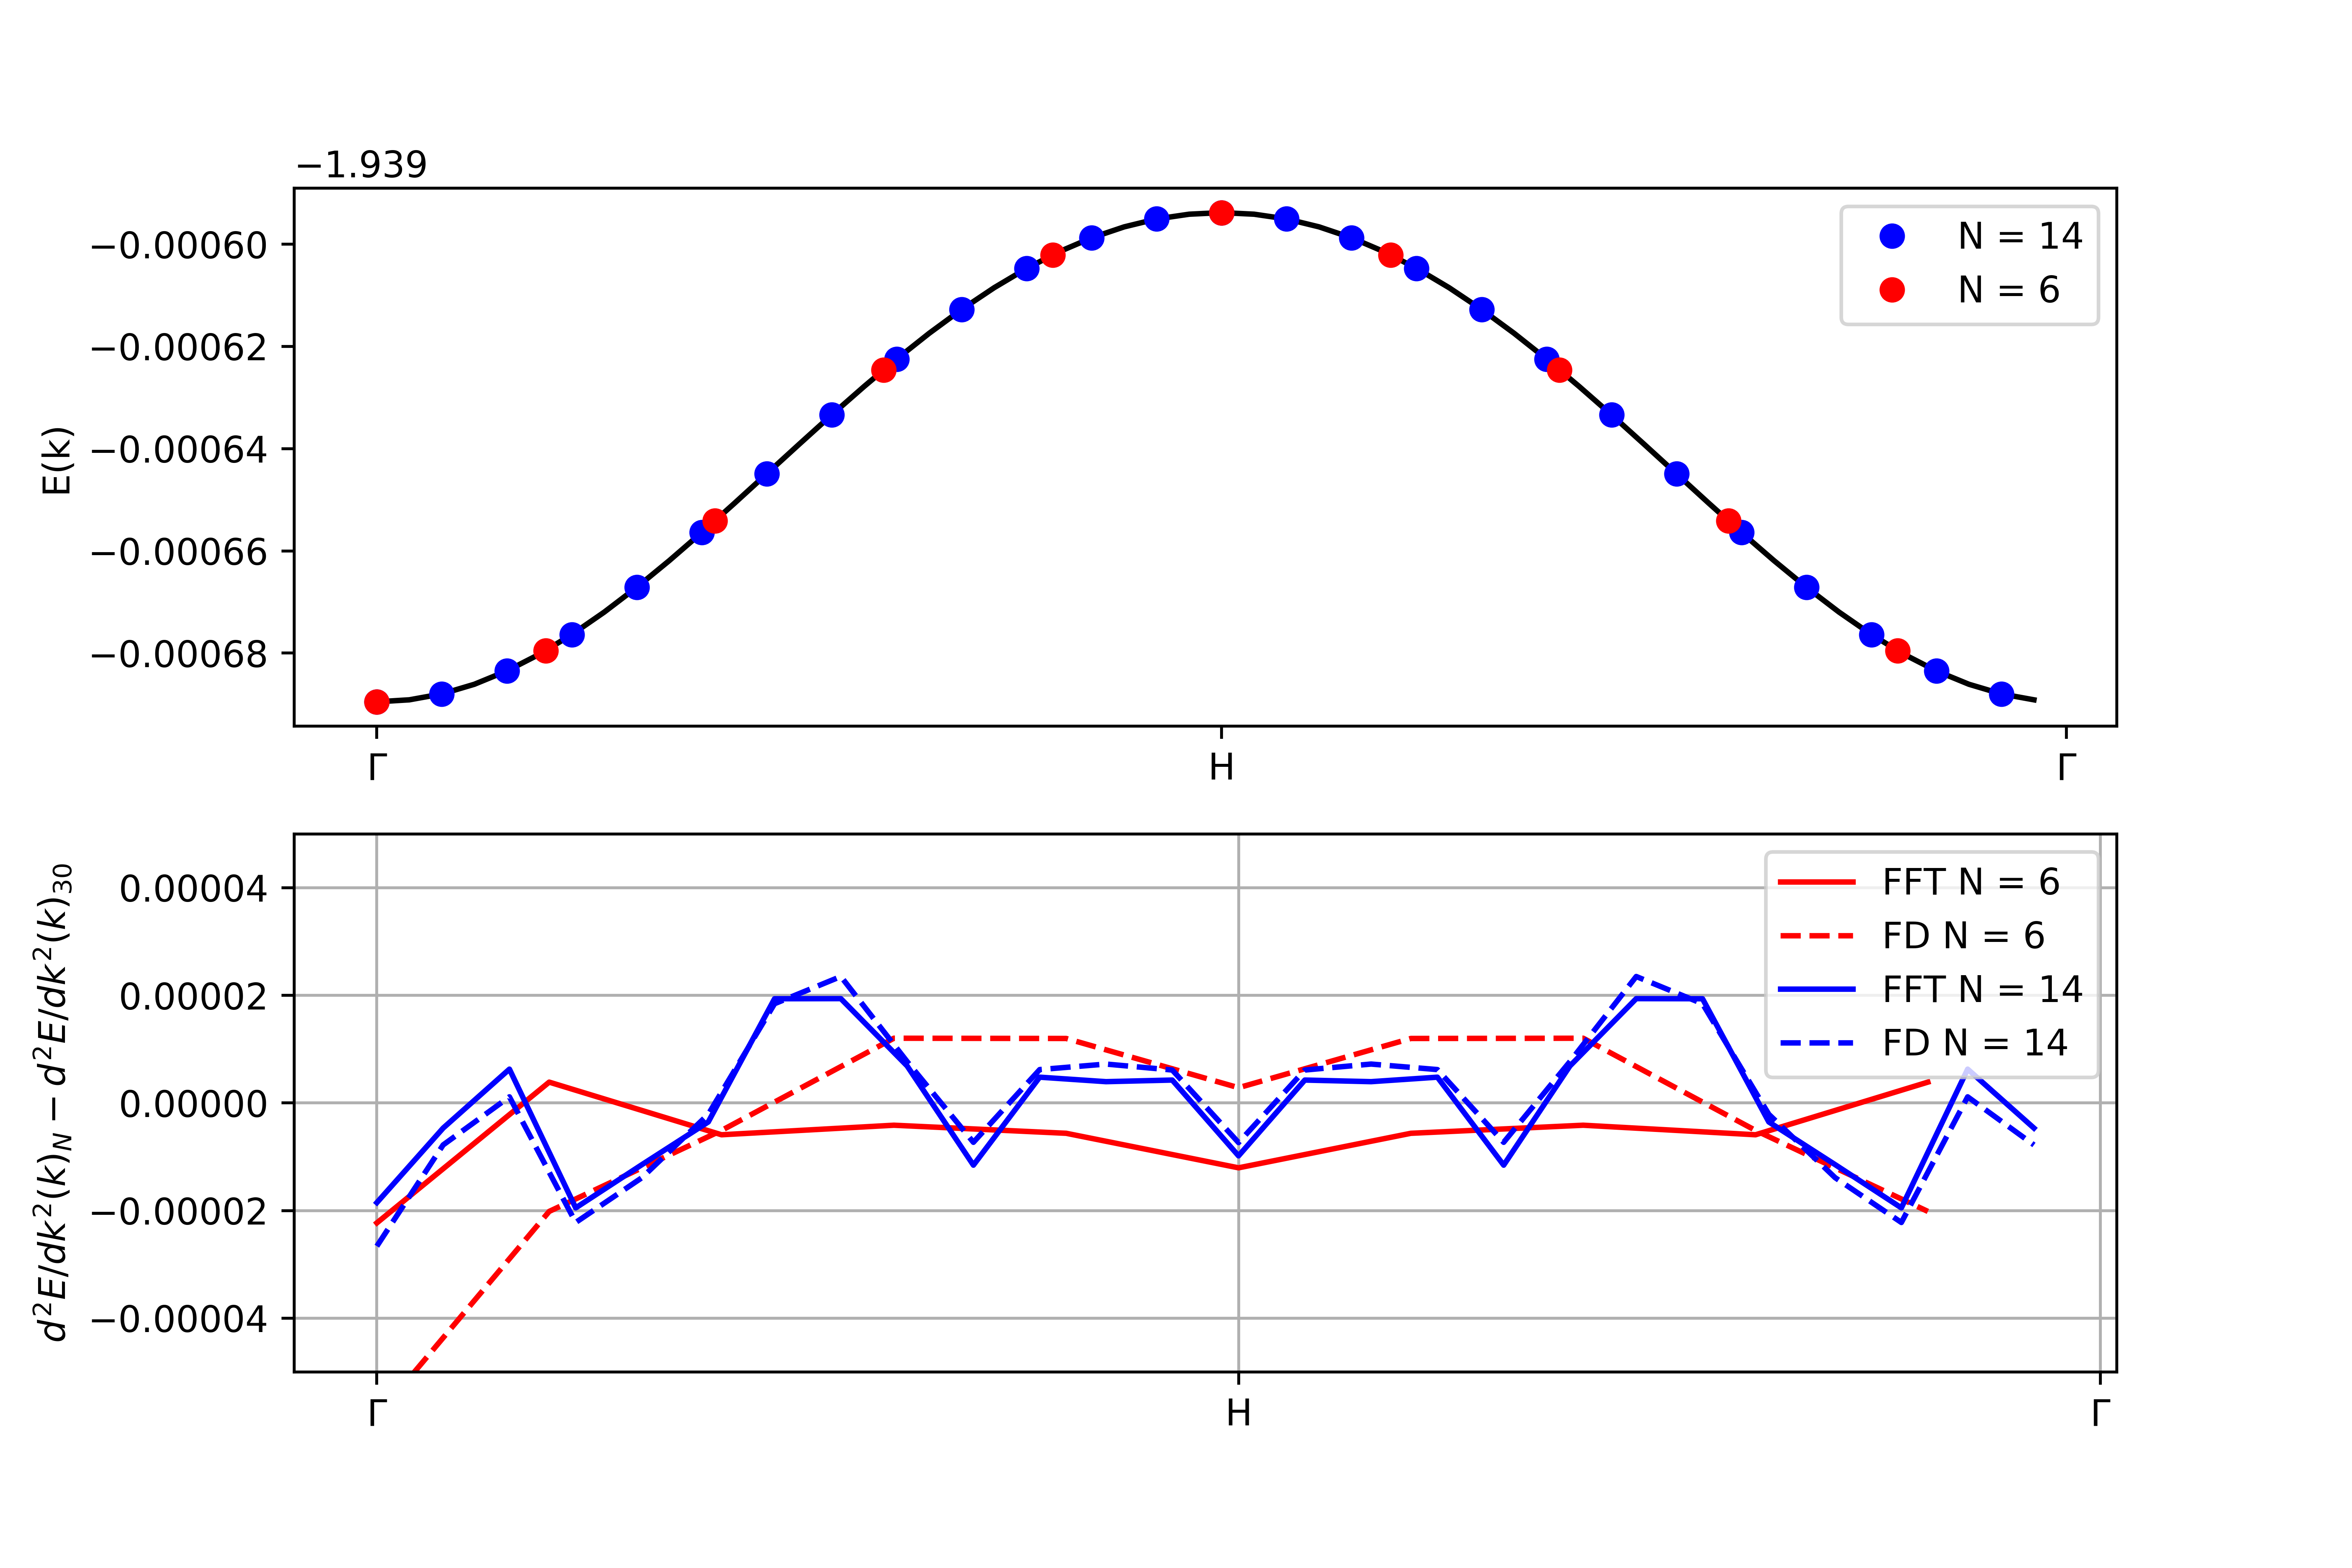
\includegraphics[width=0.7\linewidth]{christian/diff_compare.png}
    \caption{Comparison between FFT differentiation method and central finite difference method}
    \label{num_diff}
\end{figure}

When using more points, the difference between both approximation schemes is not significant. It is interesting to note, that the FFT method does not work anymore in the limit of extremely many points. In this case the derivative is dominated by Gibbs oscillations. These are most likely caused by small discontinuities in $E(\mathbf{k})$, due to basis changes inside the DFT computation.

At the current state the question remains to be answered weather the computation of $m^{*}$ and $v_g$ is useful. The number of bands, which the computation can be applied to is extremely limited. Since the bands in the data files are not labeled according to their corresponding eigenfunction but sorted by value, there are discontinuities at each point, where two bands intersect. This problem might be solved in the future. 













 %   \item Effective mass, that an electon in a crystal appears to have compared to a free %electron (due to interactions in the solid)
%    $m^{*} = \hbar^2  \left(\frac{\partial^2E(\mathbf{k})}{\partial k^2}\right)^{-1}$
%    \
%    \item Group velocity:
%    $v_{G}(\mathbf{k}) = \frac{1}{\hbar}\frac{\partial E(\mathbf{k})}{\partial \mathbf{k}}$%
%
%    
%    \item Problem: sparse k-Point mesh, but periodic band structure
%    \item Idea: Using FFT to compute accurate derivates:
%    \newline $\Leftrightarrow$ Differentiate a finite Fourier series
%    \newline $f^{(n)}(x) = \mathcal{F}^{-1}\left((ik)^n\mathcal{F}(f(x))\right)$


%%% Local Variables:
%%% mode: latex
%%% TeX-master: "../report"
%%% End:


\chapter{Conclusion}
\label{chap:conclusion}

%% JW: proofread modification v1 of PK Original ========================================
\begin{itemize}
    \item A software package was developed to visualize DFT data in an appropriate way. The data is read, extracted and visualized using the package.
    \item An API and GUI was developed which are easy to use, easy to get the
        visualization output. The visualization is physically correct and visually appealing.
    \item Additional studies of physical features are performed to derive the
        effective mass ($m\*$) and Fermi velocity($v_{fermi}$), using numerical
        differentiation techniques, which is helpful in analyzing materials
        characteristics.
    \item The Fleur output data are now easily accesible to non-experts since
        processing and visualization is done by the software.
    \item The possibility of integration of the backend into AiiDA workflows and
        the Web GUI into AiiDA Lab makes it easier for anyone to access simulation results and understand the simulation much faster.
    \item Features extracted through the simulation data can also be saved for further research and analysis.
    \item A directly executable Desktop GUI which makes it easier to use in any computer just by copying the GUI.
\end{itemize}

% % %% PK Original ========================================
% \begin{itemize}
%     \item A package to developed to visualize DFT data in an appropriate way. The data is read, extracted and visualized using the package.
%     \item An API and GUI are developed which are easy to use, easy to get the visualization output and visually appealing.
%     \item The API is used and studies data to external physical feature such as effective mass ($m\*$), Fermi Velocity($v_{fermi}$) using numerical differentiation techniques which is helpful in analyzing materials characteristics.
%     \item Fluer output data are now easily accesible to non-experts since processing and visualization done by this API.
%     \item Integrating of API and GUI into AiiDA workflow makes it easier for anyone to access this and understand the simulation much faster.
%     \item Features extracted through the simulation data can also be saved for further research and analysis.
%     \item A directly executable GUI which makes it easier to use in any computer just by copying the GUI.
% \end{itemize}


\section{Outlook}
\label{sec:outlook}

\begin{itemize}
\item Preprocessor submodule:
    \begin{itemize}
    \item Dataset dependencies for new recipes have to be explicitly stated.
        This could also be automatically resolved by type inspection.
    \item The data selection method of the output type \texttt{FleurBands} could
        be optimized even more by replacing \textit{all} numerical operations
        with \texttt{numpy} routines.
    \item In the context of general workflows, the preprocessor recipes could be
        written to serve as glue between different simulation programs. An
        example might be the conversion of a converged Fleur DFT calculation as
        a reference mean-field system input for
        \href{https://spex.readthedocs.io/en/master/spex_and_fleur.html#old-fleur}{Spex},
        another DFT code in the Jülich FLAPW code family that uses the GW
        approximation.
    \end{itemize}
\item Visualization module and Frontends:
    \begin{itemize}
    \item The fact that the Web Frontend is only in experimental stage and not
        yet publishable as a standalone app is a drawback. However it is hoped,
        that the instructions for that in the developer section of the manual
        \vref{for-developers} will help to realize that milestone more easily. 
    \item The other open issues mentionend in the developer section can be addressed to improve the user
        experience and the performance, yet they do not compromise the frontend
        usage significantly.
    \item PyViz Param \cite{pyviz-param} makes it possible to decouple the
        formal description of a particular GUI from the GUI library used. This
        would serve to separate interface and implementation like it is done in
        the preprocessor and visualization submodules.
    \end{itemize}
\end{itemize}


%%% Local Variables:
%%% mode: latex
%%% TeX-master: "../report"
%%% End:


\appendix

% % Original template (biblatex):
% \bibliographystyle{authoryear-fr}
% \bibliographystyle{authoryear}
% \bibliography{references}

% Adapted template (biber):
\printbibliography

% \clearpage

%%%%%%%%%%%%%%%% 
%%% Abstract %%%
%%%%%%%%%%%%%%%% 

\thispagestyle{empty}

\vspace*{\fill}
\noindent\rule[2pt]{\textwidth}{0.5pt}\\
{\textbf{Abstract ---}}
In this project, the raw data of the DFT simulations from Fleur are read, pre-processed and stored in suitable variables, then  extracted various features from the data from the DFT simulations such as Fermi velocity, Effective mass. Then this data is visualized using suitable color pots for a physicist to understand the plots, material characteristics using the plots. This API is converted into a frontend GUI for easier use in future. The overall project helps physicists to solve their problem of reading the DFT simulations data.

{\textbf{Keywords}}
Fleur, DFT Simulations, visualization, Front end GUI, Feature extraction.
\\
\noindent\rule[2pt]{\textwidth}{0.5pt}
\begin{center}
    AICES\\
    Schinkelstr. 2\\
    Rogowski Building\\
    4th Floor\\
    52062 Aachen    
\end{center}
\vspace*{\fill}

%%% Local Variables:
%%% mode: latex
%%% TeX-master: "report"
%%% End:
                % original template

\end{document}
%%% Local Variables:
%%% mode: latex
%%% TeX-master: t
%%% End:
